%!TEX TS-program = xelatex
%!TEX options = -aux-directory=Debug -shell-escape -file-line-error -interaction=nonstopmode -halt-on-error -synctex=1 "%DOC%"
\documentclass{article}
\input{LaTeX-Submodule/template.tex}

% Additional packages & macros
\DeclareMathOperator*{\argmax}{arg\ max}

% Header and footer
\newcommand{\unitName}{Digital Signals and Image Processing}
\newcommand{\unitTime}{Semester 2, 2024}
\newcommand{\unitCoordinator}{Dr Maryam Haghighat}
\newcommand{\documentAuthors}{Tarang Janawalkar}

\fancyhead[L]{\unitName}
\fancyhead[R]{\parbox[b]{9cm}{\raggedleft\leftmark}}
\fancyfoot[C]{\thepage}

% Copyright
\usepackage[
    type={CC},
    modifier={by-nc-sa},
    version={4.0},
    imagewidth={5em},
    hyphenation={raggedright}
]{doclicense}

\date{}

\begin{document}
%
\begin{titlepage}
    \vspace*{\fill}
    \begin{center}
        \LARGE{\textbf{\unitName}} \\[0.1in]
        \normalsize{\unitTime} \\[0.2in]
        \normalsize\textit{\unitCoordinator} \\[0.2in]
        \documentAuthors
    \end{center}
    \vspace*{\fill}
    \doclicenseThis
    \thispagestyle{empty}
\end{titlepage}
\newpage
%
\tableofcontents
\newpage
%
\section{Digital Image Processing}
Digital image processing is the processing of images on a digital
system using algorithms. A digital image is a binary representation of
visual data that is composed of a finite number of elements, each with
a particular location and value.

Image processing methods can be divided into two categories:
\begin{itemize}
    \item Methods where the input and output are images.
    \item Methods where the input is an image and the output is some
          information extracted from the image.
\end{itemize}
\subsection{Elements of Visual Perception}
The human visual system has influenced and contributed to many
advancements in image processing. The human eye has light receptors
called rods and cones. Humans have around \numrange{6}{7} million cones
in each eye that are highly sensitive to colour and fine details. On
the other hand, there are a total of \numrange{75}{150} million rods
across both eyes, that are sensitive to low levels of illumination.
\subsubsection{Image Formation}
Photo camera lenses are fixed in focal length and they focus at various
distances by varying the distance between the lens and imaging plane
(film/chip). The human eye works in the opposite way, where the
distance between the lens and the imaging plane (retina) is fixed, but
the focal length for focus is varied by changing the shape of the lens.
\subsubsection{Brightness Adaptation and Discrimination}
The human eye is capable of discriminating between a wide range of
intensity levels. This range of light intensity levels is on the order
of \(10^{10}\).
\subsection{Image Generation Components}
There are three components to image generation:
\begin{itemize}
    \item \textbf{Object}: The object being imaged.
    \item \textbf{Energy Source}: The source of energy that illuminates the object.
    \item \textbf{Sensor}: The sensor that detects the energy reflected from the object.
\end{itemize}
Depending on the properties of the energy source and object material and
geometry, the emitted energy can be reflected, transmitted, or absorbed.
\subsubsection{Electromagnetic Spectrum}
The main source of energy for imaging is electromagnetic (EM)
radiation. EM radiation consists of propagating sinusoidal waves
characterised by their oscillating frequency \(f\). Using Planck's
equation, the energy of a photon can be calculated as
\begin{equation*}
    E = hf
\end{equation*}
where \(h = \qty{6.62607015E-34}{J.s}\) is Planck's constant and \(f\) is the frequency of the wave.
Given the speed of light \(c = \qty{299792458}{m.s^{-1}}\), we can also calculate the energy using
\begin{equation*}
    E = \frac{hc}{\lambda}.
\end{equation*}
The EM spectrum is divided into regions based on the frequency of the
waves. The visible light spectrum is a small part of the EM spectrum
that is visible to the human eye. The visible light spectrum ranges
from \qty{380}{nm} to \qty{700}{nm}. Earth's atmosphere also blocks
certain parts of the EM spectrum, such as short wavelength UV and X-rays.

\textbf{Perceived colour} (hue) is related to the wavelength of light,
while the \textbf{brightness} is related to the intensity of the
radiation.
\subsubsection{Image Sensors}
Image sensors capture a specific range of the EM spectrum, for example:
\begin{itemize}
    \item RGB sensors capture the visible light spectrum.
    \item Infrared sensors capture the infrared spectrum.
    \item X-ray sensors capture the X-ray spectrum.
    \item Ultraviolet sensors capture the ultraviolet spectrum.
\end{itemize}
\subsubsection{Human Perception}
Human perception is context-dependent. Perceived intensity around
regions of discontinuous intensity appear to undershoot and overshoot
around the boundary (see Mach band effect). The eye can also fill in
non-existing information and wrongly perceive geometrical properties of
objects. To produce a powerful vision system, we need both a powerful
image sensor and image processor to extract useful information from an
image.
\subsection{Image Sensing and Acquisition}
Image sensing is the process of transforming illuminated energy into a
digital image. The process involves the following steps:
\begin{enumerate}
    \item Convert the illuminated energy into an electrical signal.
    \item Digitize the electrical signal to obtain a digital image.
\end{enumerate}
\subsubsection{Image Sensing Modalities}
Image sensing is done using three principal modalities:
\begin{itemize}
    \item \textbf{Single Sensing Element}: A single sensor that
          captures the energy. For example, a photodiode. To
          generate 2D images, the sensor must be appropriately
          displaced in the \(x\) and \(y\) directions.
    \item \textbf{Line Sensor}: A sensor that captures energy
          along a line. To generate 2D images, the sensor must
          be displaced in the direction perpendicular to the
          line.
    \item \textbf{Array Sensor}: A sensor that captures energy
          in a 2D array. The sensor is divided into rows and
          columns, with each element capturing energy at a
          specific location. A typical arrangement is the
          \textbf{CCD} (Charge Coupled Device) sensor.
\end{itemize}
\subsubsection{Image Formation}
Let us denote the intensity of a monochrome image by the 2-dimensional
function
\begin{equation*}
    \ell = f\left( x,\: y \right)
\end{equation*}
where \(x\) and \(y\) represent the spatial coordinates captured by the
sensor, and \(f\) is a scalar function of the intensity of the energy
radiated by a physical source. As such, this function is non-negative
and finite:
\begin{equation*}
    0 \leqslant \ell \leqslant \infty.
\end{equation*}
\(f\) is characterised by two components:
\begin{itemize}
    \item \textbf{Illumination}: The amount of source illumination incident on the
          scene \(i\left( x,\: y \right)\). Here \(0 \leqslant i\left( x,\: y \right) < \infty\).
    \item \textbf{Reflectance}: The amount of illumination reflected by
          the objects on the scene \(r\left( x,\: y \right)\). Here
          \(0 \leqslant r\left( x,\: y \right) \leqslant 1\).
\end{itemize}
Therefore, we can describe the image formation process as
\begin{equation*}
    f\left( x,\: y \right) = i\left( x,\: y \right) r\left( x,\: y \right),
\end{equation*}
where \(r = 0\) implies total absorption, while \(r = 1\) implies total reflectance.
For monochrome images, we can define the minimum and maximum intensity
values as \(L_{\text{min}}\) and \(L_{\text{max}}\), respectively,
where
\begin{equation*}
    L_{\text{min}} \leqslant \ell \leqslant L_{\text{max}}, \quad L_{\text{min}} = i_{\text{min}} r_{\text{min}}, \quad L_{\text{max}} = i_{\text{max}} r_{\text{max}}.
\end{equation*}
The range of intensity values \(\interval{L_{\text{min}}}{L_{\text{max}}}\)
is called the \textbf{intensity/grey scale}. Commonly, this interval is
transformed to the interval \(\interval{0}{L-1}\), where \(L\) is the
number of intensity levels.
\subsection{Image Sampling and Quantisation}
\textbf{Image sampling} is the process of sampling discrete points in a
continuous image. Regardless of the sensor arrangement, the image is
sampled at a fixed rate in the \(x\) and \(y\) directions and the
resulting points are called \textbf{pixels}. These pixels are stored in
an array that is \(M \times N\) in size, where \(M\) is the number of
rows and \(N\) is the number of columns, arranged as shown below:
\begin{equation*}
    \symbf{X} =
    \begin{bmatrix}
        x_{00}    & x_{01}    & \cdots & x_{0,N-1}   \\
        x_{10}    & x_{11}    & \cdots & x_{1,N-1}   \\
        \vdots    & \vdots    & \ddots & \vdots      \\
        x_{M-1,0} & x_{M-1,1} & \cdots & x_{M-1,N-1}
    \end{bmatrix}
\end{equation*}
\textbf{Image quantisation} is the process of converting the continuous
intensity values of an image to discrete values. The number of
intensity levels \(L\) is determined by the number of bits used to
represent each pixel. The number of intensity levels is given by
\begin{equation*}
    L = 2^k,
\end{equation*}
where \(k\) is the bit depth. Thus the quantised intensity values will
range from \(\interval{0}{L-1}\). The \textbf{quality} of an image is
determine by the number of discrete intensity levels used in both
sampling and quantisation.
\subsubsection{Dynamic Range and Contrast}
The \textbf{dynamic range} of an image is the ratio of the maximum
intensity value to the minimum intensity value:
\begin{equation*}
    \text{Dynamic Range} = \frac{L_{\text{max}}}{L_{\text{min}}} = \frac{i_{\text{max}} r_{\text{max}}}{i_{\text{min}} r_{\text{min}}}.
\end{equation*}
The upper limit is determined by the sensor's saturation level, while
the lower limit is determined by the sensor's noise level. The
\textbf{contrast} of an image is the difference in intensity between the
brightest and darkest regions of the image:
\begin{equation*}
    \text{Contrast} = L_{\text{max}} - L_{\text{min}} = i_{\text{max}} r_{\text{max}} - i_{\text{min}} r_{\text{min}}.
\end{equation*}
\begin{itemize}
    \item A \textbf{high} dynamic range implies a large difference
          between the brightest and darkest regions of the image, and
          therefore high contrast.
    \item A \textbf{low} dynamic range implies a small difference
          between the brightest and darkest regions of the image, and
          therefore low contrast.
\end{itemize}
\subsubsection{Spatial and Intensity Resolution}
The \textbf{spatial resolution} of an image is a measure of the
smallest discernible detail in an image, measured as the number of
pixels per unit area (dots per inch). In some images, sampling an image
at a low rate can result in \textbf{aliasing}, where high-frequency
components are incorrectly represented as low-frequency components (see
the Moiré pattern).

The \textbf{intensity resolution} of an image is the smallest
discernible change in intensity level, which is related to the number
of intensity levels used to represent the image, for example, 8-bit and
10-bit images. Choosing a low number of intensity levels can result in
quantisation noise, where intensity levels are incorrectly represented.
\subsubsection{Image Interpolation}
Image interpolation is the process of estimating the intensity values
of pixels between the sampled points. Interpolation is used to increase
and decrease the resolution of an image for resampling and resizing.
Common interpolation methods include:
\begin{itemize}
    \item \textbf{Nearest Neighbour}: The intensity value of the nearest
          pixel is used to estimate the intensity value of the pixel.
    \item \textbf{Bilinear}: The intensity value of the nearest four
          pixels is used to estimate the intensity value of the pixel.
    \item \textbf{Bicubic}: The intensity value of the nearest sixteen
          pixels is used to estimate the intensity value of the pixel.
\end{itemize}
\subsection{Relationships Between Pixels}
The following sections will define some common sets that are used to
describe relationships between pixels in an image.
\subsubsection{Neighbours of a Pixel}
The \textbf{neighbours} of a pixel \(\symbf{p} = \left( x,\: y
\right)\) are the pixels that are adjacent to \(\symbf{p}\).
\begin{itemize}
    \item The \textbf{4-neighbours} of \(\symbf{p}\) are defined as the
          pixels that are adjacent to \(\symbf{p}\) in the
          \textbf{cardinal} directions:
          \begin{equation*}
              \symbf{N}_4\left( \symbf{p} \right) = \left\{ \left( x,\: y-1 \right), \left( x-1,\: y \right), \left( x+1,\: y \right), \left( x,\: y+1 \right) \right\},
          \end{equation*}
    \item The \textbf{diagonal-neighbours} of \(\symbf{p}\) are defined
          as the pixels that are adjacent to \(\symbf{p}\) in the
          \textbf{diagonal} directions:
          \begin{equation*}
              \symbf{N}_D\left( \symbf{p} \right) = \left\{ \left( x-1,\: y-1 \right), \left( x+1,\: y-1 \right), \left( x-1,\: y+1 \right), \left( x+1,\: y+1 \right) \right\},
          \end{equation*}
    \item The \textbf{8-neighbours} of \(\symbf{p}\) are defined as the
          pixels that are adjacent to \(\symbf{p}\) in both the
          \textbf{cardinal} and \textbf{diagonal} directions:
          \begin{equation*}
              \symbf{N}_8\left( \symbf{p} \right) = \symbf{N}_4\left( \symbf{p} \right) \cup \symbf{N}_D\left( \symbf{p} \right).
          \end{equation*}
\end{itemize}
\subsubsection{Adjacency and Connectivity}
Two pixels \(\symbf{p}\) and \(\symbf{q}\) are \textbf{adjacent} if
they are neighbours and their intensity values are similar or belong to
the same set of values \(V\) based on a threshold. This can occur in
one of three ways:
\begin{itemize}
    \item \textbf{4-Adjacency} when \(\symbf{q} \in \symbf{N}_4\left( \symbf{p} \right)\).
    \item \textbf{8-Adjacency} when \(\symbf{q} \in \symbf{N}_8\left( \symbf{p} \right)\).
    \item \textbf{M-Adjacency} when \(\symbf{q} \in \symbf{N}_4\left( \symbf{p} \right)\) \textbf{or} \(\symbf{q} \in \symbf{N}_D\left( \symbf{p} \right)\) \textbf{and} \(\symbf{N}_4\left( \symbf{p} \right) \cap \symbf{N}_4\left( \symbf{q} \right) = \emptyset\).
          This statement avoids double-counting an adjacency when
          \(\symbf{q}\) is a diagonal neighbour of \(\symbf{p}\) while
          another cardinal neighbour exists between \(\symbf{p}\) and
          \(\symbf{q}\). Consider the binary example with \(\symbf{p},\symbf{q},\symbf{r} \in V = \left\{ 1 \right\}\):
          \begin{equation*}
              \begin{bmatrix}
                  0 & \symbf{r} & \symbf{q} \\
                  0 & \symbf{p} & 0         \\
                  0 & 0         & 0
              \end{bmatrix}
              .
          \end{equation*}
          Here we do not consider \(\symbf{p}\) and \(\symbf{q}\) to be
          M-adjacent, as \(\symbf{p}\) and \(\symbf{q}\) are already
          adjacent through \(\symbf{r}\).
\end{itemize}
A \textbf{path} (or curve) between two pixels \(\symbf{p}\) and
\(\symbf{q}\) is a sequence of \(n+1\) pixels \(\left( \symbf{p}_0, \symbf{p}_1,
\ldots, \symbf{p}_n \right)\) such that \(\symbf{p}_0 = \symbf{p}\) and
\(\symbf{p}_n = \symbf{q}\), where \(\symbf{p}_i\) is adjacent to
\(\symbf{p}_{i+1}\) for \(i = 0, 1, 2, \ldots, n-1\). This path is said
to have length \(n\), and is \textit{closed} if \(\symbf{p}_0 = \symbf{p}_n\).
\subsubsection{Connectivity}
Consider a subset of pixels in an image \(S\) with \(\symbf{p},
\symbf{q} \in S\).
\begin{itemize}
    \item \(\symbf{p}\) and \(\symbf{q}\) are \textbf{connected} if
          there exists a path between \(\symbf{p}\) and \(\symbf{q}\) such
          that all pixels in the path are in \(S\).
    \item The set of pixels connected to \(\symbf{p}\) in \(S\) form a
          \textbf{connected component}.
    \item If \(S\) only consists of \textit{one} connected component,
          then \(S\) is said to be a \textbf{connected set} and is
          called a \textbf{region} \(R\).
\end{itemize}
Two regions \(R_1\) and \(R_2\) are adjacent if their union forms a
connected set, i.e., another region. Regions that are not adjacent are
said to be \textbf{disjoint}.
\subsection{Distance Metrics}
The \textbf{distance} between two pixels \(\symbf{p}\) and
\(\symbf{q}\) can be measured using a variety of metrics. The most
common metrics are:
\begin{itemize}
    \item \textbf{Euclidean distance}:
          \begin{equation*}
              d\left( \symbf{p},\: \symbf{q} \right) = \sqrt{\left( x_p - x_q \right)^2 + \left( y_p - y_q \right)^2}.
          \end{equation*}
    \item \textbf{Manhattan (D4) distance} (or city-block distance):
          \begin{equation*}
              d_4\left( \symbf{p},\: \symbf{q} \right) = \abs{x_p - x_q} + \abs{y_p - y_q}.
          \end{equation*}
    \item \textbf{Chessboard (D8) distance} (or maximum distance):
          \begin{equation*}
              d_8\left( \symbf{p},\: \symbf{q} \right) = \max\left( \abs{x_p - x_q},\: \abs{y_p - y_q} \right).
          \end{equation*}
\end{itemize}
In general, any metric \(d\) that satisfies the following properties is a
\textbf{distance metric}:
\begin{itemize}
    \item The distance from a point to itself is zero:
          \begin{equation*}
              d\left( \symbf{p},\: \symbf{p} \right) = 0.
          \end{equation*}
    \item \textbf{Positivity}: The distance between two distinct points is always positive:
          \begin{equation*}
              d\left( \symbf{p},\: \symbf{q} \right) > 0 : \symbf{p} \neq \symbf{q}.
          \end{equation*}
    \item \textbf{Symmetry}: The distance between two points is always the same regardless of ordering:
          \begin{equation*}
              d\left( \symbf{p},\: \symbf{q} \right) = d\left( \symbf{q},\: \symbf{p} \right).
          \end{equation*}
    \item The Triangle Inequality is satisfied:
          \begin{equation*}
              d\left( \symbf{p},\: \symbf{q} \right) \leq d\left( \symbf{p},\: \symbf{r} \right) + d\left( \symbf{r},\: \symbf{q} \right).
          \end{equation*}
\end{itemize}
for all \(\symbf{p},\: \symbf{q},\: \symbf{r}\) in this metric space.
\subsection{Mathematical Operations}
\subsubsection{Element-wise Operations}
Given two images \(\symbf{X}\) and \(\symbf{Y}\) of equal dimensions,
an element-wise operation is an operation that is applied to each pixel
in the image. Suppose we wish to apply the binary operation \(\otimes\)
on \(\symbf{X}\) and \(\symbf{Y}\). The resulting image \(\symbf{Z}\)
is given by
\begin{equation*}
    \symbf{Z} = \symbf{X} \otimes \symbf{Y} =
    \begin{bmatrix}
        x_{00} \otimes y_{00}       & x_{01} \otimes y_{01}       & \cdots & x_{0,N-1} \otimes y_{0,N-1}     \\
        x_{10} \otimes y_{10}       & x_{11} \otimes y_{11}       & \cdots & x_{1,N-1} \otimes y_{1,N-1}     \\
        \vdots                      & \vdots                      & \ddots & \vdots                          \\
        x_{M-1,0} \otimes y_{M-1,0} & x_{M-1,1} \otimes y_{M-1,1} & \cdots & x_{M-1,N-1} \otimes y_{M-1,N-1}
    \end{bmatrix}
\end{equation*}
Here the operator \(\otimes\) can represent any binary operation, such
as addition, subtraction, multiplication, or division.
\subsubsection{Linear Operations}
The operator \(H\) is a linear operation if it satisfies the following
property:
\begin{equation*}
    H\left[ a\symbf{X} + b\symbf{Y} \right] = aH\left[ \symbf{X} \right] + bH\left[ \symbf{Y} \right],
\end{equation*}
for images \(\symbf{X}\) and \(\symbf{Y}\), where \(a\) and \(b\) are constants.
\subsubsection{Spatial Operations}
The operator \(T\) is a spatial operation if the output pixel value is
determined by the values of pixels in the neighbourhood of any input
pixel. \(T\) can be categorised as one of three types of spatial
operations:
\begin{itemize}
    \item \textbf{Pointwise}: The output pixel value is
          determined by the value of the input pixel only.
    \item \textbf{Neighbourhood}: The output pixel value is
          determined by the value of the input pixel and any
          neighbouring pixels.
    \item \textbf{Global}: The output pixel value is
          determined by the value of pixels in the entire image.
    \item \textbf{Geometric}: The output pixel value is
          determined by the spatial location of the pixel.
\end{itemize}
\section{Intensity Transformations \& Spatial Filters}
\subsection{Intensity Transformations}
An intensity transform aims to modify the contrast of an image by
changing the range of intensity values in that image. The following
sections will define some common intensity transformations. In the
following sections let \(r\) be the input intensity and \(s\) be the
output intensity of an image.
\subsubsection{Identity Transformation}
The identity transformation is the simplest intensity transformation
which does not alter an image. It is defined as
\begin{equation*}
    s = T\left( r \right) = r.
\end{equation*}
\subsubsection{Negative Transformation}
The image negation transformation is used to invert the intensity
values of an image. It is defined as
\begin{equation*}
    s = T\left( r \right) = \left( L - 1 \right) - r,
\end{equation*}
where \(L\) is the number of intensity levels in the image.
\subsubsection{Logarithmic Transformation}
The logarithmic transformation is used to enhance darker regions of an
image by compressing brighter regions. It is defined as
\begin{equation*}
    s = T\left( r \right) = c \log{\left( 1 + r \right)},
\end{equation*}
where \(c\) is a constant that scales the intensity values of the image.
\subsubsection{Power-Law (Gamma) Transformation}
The power-law transformation is used to correct the gamma of an image,
either by enhancing or reducing dark or bright regions. It can be
thought of as a generalisation of the logarithmic transformation. It is
defined as
\begin{equation*}
    s = T\left( r \right) = c r^\gamma,
\end{equation*}
where \(c\) is a constant that scales the intensity values of the image
and \(\gamma\) is the gamma value.
\begin{itemize}
    \item When \(\gamma < 1\), the transformation enhances the darker
          regions of the image, while compressing the brighter regions.
    \item When \(\gamma > 1\), the transformation enhances the brighter
          regions of the image, while compressing the darker regions.
\end{itemize}
\subsubsection{Piecewise-Linear Transformation}
Piecewise-linear transformations are used to enhance the contrast of
specific regions of an image. Some common piecewise-linear
transformations include:
\begin{itemize}
    \item \textbf{Contrast Stretching}: Enhances the contrast of an
          image by stretching the intensity values to the full range of
          intensity levels.
    \item \textbf{Intensity Level Slicing}: Enhances the contrast of
          specific regions of an image by setting the intensity values
          of other regions to zero or by leaving them unchanged.
    \item \textbf{Bit-Plane Slicing}: Highlights the contribution made
          to image appearance by specific bits in the image.
\end{itemize}
\subsection{Histogram Processing}
Histograms are used to visualise the distribution of intensity values
in an image. Given an image \(\symbf{X} \in \interval{0}{L-1}^{M \times
N}\), the histogram \(h_{\symbf{X}}\left( k \right)\) is defined as
\begin{equation*}
    h_{\symbf{X}}\left( k \right) = n_k,
\end{equation*}
where \(n_k\) is the number of pixels in the image with intensity value
\(k\). If we normalise these values, we find the probability of
obtaining a pixel with intensity value \(k\):
\begin{equation*}
    p_{\symbf{X}}\left( k \right) = \frac{n_k}{MN}.
\end{equation*}
It follows that
\begin{equation*}
    \sum_{k=0}^{L-1} p_{\symbf{X}}\left( k \right) = 1.
\end{equation*}
\subsubsection{Histogram Equalisation}
Histogram equalisation is a method used to spread the most frequent
intensity values in an image to the full range of intensity levels,
thereby achieving a more uniform distribution of intensity values. To
do this, we will use the following transformation that maps the
cumulative distribution function of an input image \(\symbf{X}\) to the
cumulative distribution function of a uniform distribution:
\begin{equation*}
    s = T\left( r \right) = \left( L - 1 \right) \sum_{j=0}^{r} p_{\symbf{X}}\left( j \right) = \frac{L - 1}{MN} \sum_{j=0}^{r} n_j.
\end{equation*}
\subsubsection{Histogram Matching}
In some cases, we wish to match the histogram of \(\symbf{X}\) to the
histogram of another image \(\symbf{Y}\). To do so, consider the
histogram equalisation of \(\symbf{Y}\) with intensity values \(z\):
\begin{equation*}
    s = G\left( z \right) = \left( L - 1 \right) \sum_{j=0}^{z} p_{\symbf{Y}}\left( j \right) = \frac{L - 1}{MN} \sum_{j=0}^{z} n_j.
\end{equation*}
Thus we have the mapping:
\begin{equation*}
    T: r \mapsto s \quad \text{and} \quad G: z \mapsto s.
\end{equation*}
As both \(T\) and \(G\) map to the same equalised space, we can define
the transformation \(z = H\left( r \right)\) that maps the histogram of
\(\symbf{X}\) to the histogram of \(\symbf{Y}\) as
\begin{equation*}
    z = H\left( r \right) = G^{-1}\left( T\left( r \right) \right) = G^{-1}\left( s \right).
\end{equation*}
\subsection{Spatial Filtering}
Spatial filtering is the process of creating a new image by applying a
mask (or kernel, template or window) to each pixel in an image. This
new pixel value is determined by the intensity values of the pixels in
the neighbourhood of the original pixel. The mask is defined as a \(m
\times n\) matrix \(\symbf{W}\) with elements \(w_{ij}\) that represent
the weights of the pixels in the neighbourhood of the pixel being
processed. For convenience, \(m\) and \(n\) are typically odd integers.

The output pixel value is given by the weighted sum of the intensity
values of the pixels in the neighbourhood of the pixel. This can be
done using one of two operations:
\begin{itemize}
    \item \textbf{Correlation}: The mask is shifted across the image
          and the weighted sum is calculated at each position.
    \item \textbf{Convolution}: The mask is first flipped horizontally
          and vertically before it is shifted across the image.
\end{itemize}
\subsubsection{Correlation}
The \(\left( i,\: j \right)\)th element of the correlation of an image
\(\symbf{X}\) with a mask \(\symbf{W}\) is defined as
\begin{equation*}
    y_{ij} = \symbf{W} \star \symbf{X} = \sum_{s = -a}^a \sum_{t = -b}^b w_{st} x_{i+s, j+t}
\end{equation*}
for \(a = \frac{m-1}{2}\) and \(b = \frac{n-1}{2}\).
\subsubsection{Convolution}
The \(\left( i,\: j \right)\)th element of the convolution of an image
\(\symbf{X}\) with a mask \(\symbf{W}\) is defined as
\begin{equation*}
    y_{ij} = \symbf{W} \ast \symbf{X} = \sum_{s = -a}^a \sum_{t = -b}^b w_{st} x_{i-s, j-t}
\end{equation*}
for \(a = \frac{m-1}{2}\) and \(b = \frac{n-1}{2}\).
\subsubsection{Padding}
For masks larger than \(1 \times 1\), the indices \(w_{st}\) will
exceed the bounds of the image \(\symbf{X}\). To prevent this, the
image is often padded with an additional border of pixels. Common
padding methods include:
\begin{itemize}
    \item \textbf{Zero Padding}: The border is padded with zeros.
    \item \textbf{Boundary Replication Padding}: The border is padded with the
          intensity values of the nearest pixel.
    \item \textbf{Reflection Padding}: The border is padded with the
          intensity values of reflected pixels (one pixel away from the
          border).
\end{itemize}
\subsubsection{Averaging Filters}
Averaging filters are used to reduce noise in an image by averaging the
intensity values of the pixels in the neighbourhood of the pixel being
processed. An averaging filter considers a continuous function of two
variables, such as the multivariable Gaussian function:
\begin{equation*}
    w_{st} = \frac{1}{2\pi\sigma^2} \exp{\left( -\frac{s^2 + t^2}{2\sigma^2} \right)}.
\end{equation*}
\subsubsection{Smoothing Linear Filters}
Smoothing filters are used to reduce noise in an image by averaging the
intensity values of the pixels in the neighbourhood of the pixel being
processed. A general implementation for filtering an \(M \times N\)
image with a \textbf{weighted averaging filter} of size \(m \times n\)
is defined as:
\begin{equation*}
    y_{ij} = \frac{\sum_{s = -a}^a \sum_{t = -b}^b w_{st} x_{i+s,j+t}}{\sum_{s = -a}^a \sum_{t = -b}^b w_{st}},
\end{equation*}
\subsubsection{Order-Statistic Non-Linear Filters}
Order-statistic filters are used to reduce noise in an image by
replacing the intensity value of a pixel with the median, maximum, or
minimum intensity value of the pixels in the neighbourhood of the pixel
being processed. Median filters have good noise-reduction capabilities
with less smoothing and are used to remove impulse or salt-and-pepper
noise.
\subsubsection{Sharpening Filters}
Sharpening filters are used to enhance edges and discontinuities in an
image. One technique is to consider the Laplacian of the image
\(f\left( x,\: y \right)\):
\begin{equation*}
    \nabla^2 f = \pdv[order=2]{f}{x} + \pdv[order=2]{f}{y}.
\end{equation*}
For discrete images, we will use the first-order forward difference
approximation:
\begin{align*}
    \pdv{f}{x} & = f\left( x + 1,\: y \right) - f\left( x,\: y \right)  \\
    \pdv{f}{y} & = f\left( x,\: y + 1 \right) - f\left( x,\: y \right),
\end{align*}
and the second-order central difference approximation:
\begin{align*}
    \pdv[order=2]{f}{x} & = f\left( x + 1,\: y \right) - 2f\left( x,\: y \right) + f\left( x - 1,\: y \right)  \\
    \pdv[order=2]{f}{y} & = f\left( x,\: y + 1 \right) - 2f\left( x,\: y \right) + f\left( x,\: y - 1 \right).
\end{align*}
The Laplacian allows us to identify transitions in intensity values
across an image by creating a filter with one of the following masks:
\begin{equation*}
    \symbf{W} =
    \begin{bmatrix}
        0 & 1  & 0 \\
        1 & -4 & 1 \\
        0 & 1  & 0
    \end{bmatrix}
    \quad \text{or} \quad \symbf{W} =
    \begin{bmatrix}
        0  & -1 & 0  \\
        -1 & 4  & -1 \\
        0  & -1 & 0
    \end{bmatrix}
    ,
\end{equation*}
where the first mask will sharpen the image, while the second mask will
sharpen the negative of the image. In general, we can sharpen edges by
adding the Laplacian to the original image:
\begin{equation*}
    g\left( x,\: y \right) = f\left( x,\: y \right) + c \nabla^2 f\left( x,\: y \right),
\end{equation*}
where \(c = -1\) will sharpen the image, while \(c = 1\) sharpen the
negative of the image.
\subsubsection{Unsharp Masking and High-Boost Filtering}
Unsharp masking is a sharpening technique that enhances edges and
discontinuities in an image by subtracting a blurred version of the
image from the original image. The process takes the following steps:
\begin{enumerate}
    \item Blur the original image \(f\left( x,\: y \right)\).
    \item Subtract the blurred image from the original image to obtain
          the mask
          \begin{equation*}
              g_{\text{mask}}\left( x,\: y \right) = f\left( x,\: y \right) - \bar{f}\left( x,\: y \right),
          \end{equation*}
          where \(\bar{f}\left( x,\: y \right)\) is the blurred image.
    \item Add the mask to the original image to obtain a sharpened
          image:
          \begin{equation*}
              g\left( x,\: y \right) = f\left( x,\: y \right) + k g_{\text{mask}}\left( x,\: y \right), \quad k > 0.
          \end{equation*}
          where
          \begin{itemize}
              \item \(k = 1\) corresponds to unsharp masking.
              \item \(k > 1\) corresponds to high-boost filtering.
          \end{itemize}
\end{enumerate}
\section{Filtering in the Frequency Domain}
\subsection{2D Fourier Transform}
The 2D Fourier transform of an image \(f\left( x,\: y
\right)\)\footnote{\(f\) must satisfy the Dirichlet conditions for the
2D Fourier transform to exist.} is defined as
\begin{equation*}
    F\left( u,\: v \right) = \mathscr{F}\left\{ f\left( x,\: y \right) \right\} = \int_{-\infty}^{\infty} \int_{-\infty}^{\infty} f\left( x,\: y \right) e^{-j2\pi\left( ux + vy \right)} \odif{x} \odif{y},
\end{equation*}
with the inverse 2D Fourier transform defined as:
\begin{equation*}
    f\left( x,\: y \right) = \mathscr{F}^{-1}\left\{ F\left( u,\: v \right) \right\} = \int_{-\infty}^{\infty} \int_{-\infty}^{\infty} F\left( u,\: v \right) e^{j2\pi\left( ux + vy \right)} \odif{u} \odif{v}.
\end{equation*}
When \(f\) is a discrete \(M \times N\) image, the 2D discrete Fourier
transform is defined as
\begin{equation*}
    F\left( u,\: v \right) = \sum_{x = 0}^{M-1} \sum_{y = 0}^{N-1} f\left( x,\: y \right) e^{-j2\pi\left( ux/M + vy/N \right)},
\end{equation*}
with the inverse 2D discrete Fourier transform defined as
\begin{equation*}
    f\left( x,\: y \right) = \sum_{u = 0}^{M-1} \sum_{v = 0}^{N-1} F\left( u,\: v \right) e^{j2\pi\left( ux/M + vy/N \right)}.
\end{equation*}
Many properties of the Fourier transform in the 1D case extend to the 2D
case, such as linearity, symmetry, and shift properties. Notably, the
sampling theorem in 2D states that an image can be perfectly
reconstructed from its samples if the sampling rate \(f_s\) is greater
than twice the highest frequency component in the image:
\begin{equation*}
    f_s > 2f_{\text{max}}.
\end{equation*}
In 2D, this is equivalent to:
\begin{equation*}
    \frac{1}{\adif{x}} > 2 u_{\text{max}} \quad \text{and} \quad \frac{1}{\adif{y}} > 2 v_{\text{max}},
\end{equation*}
where \(u_{\text{max}}\) and \(v_{\text{max}}\) are the maximum
frequencies in the \(x\) and \(y\) directions, respectively. The
frequency of spatial and frequency samples can also be related by the
following equations:
\begin{equation*}
    \adif{u} = \frac{1}{M\adif{x}} \quad \text{and} \quad \adif{v} = \frac{1}{N\adif{y}}.
\end{equation*}
\subsection{Filtering in the Frequency Domain}
Filtering can also be performed in the frequency domain if the image
contains noise that is more easily removed when visualising the
magnitude and phase spectra of the image. In general, a filter in the
frequency domain is defined as
\begin{equation*}
    g\left( x,\: y \right) = \mathscr{F}^{-1}\left\{ H\left( u,\: v \right) F\left( u,\: v \right) \right\},
\end{equation*}
where \(H\left( u,\: v \right)\) is a filter designed to act on the
frequency spectrum of the image. Due to the lack of padding, the
horizontal or vertical edges of the resulting image may contain black
pixels, leading to inconsistent filtering. To avoid this, we can take
the following steps:
\begin{enumerate}
    \item For an image \(f\left( x,\: y \right)\) of size \(M \times
          N\), define padding parameters \(P = 2M\) and \(Q = 2N\).
    \item Form a padded image \(f_p\left( x,\: y \right)\) of size \(P
          \times Q\) by appending the necessary number of zeros to
          \(f\).\
    \item Multiply the padded image by \(\left( -1 \right)^{x + y}\) to
          centre the transform at the origin.
    \item Compute the 2D Fourier transform of the transformed padded
          image.
    \item Multiply the result by the symmetric filter \(H\left( u,\: v
          \right)\) of size \(P \times Q\) to form \(G\left( u,\: v
          \right)\).
    \item Obtain the processed image \(g_p\left( x,\: y \right) =
          \Re\left\{ \mathscr{F}^{-1}\left\{ G\left( u,\: v \right)
          \right\} \right\} \left( -1 \right)^{x + y}\).
    \item Obtain the final processed image \(g\left( x,\: y \right)\)
          by cropping the processed image to the original size \(M
          \times N\), which is in the top-left corner of the processed
          image.
\end{enumerate}
\subsection{Image Smoothing}
\subsubsection{Ideal Low-Pass Filters}
An ideal low-pass filter passes all frequencies within a circle of
radius \(D_0\) from the origin and suppresses all frequencies outside
of this circle, without attenuation:
\begin{equation*}
    H\left( u,\: v \right) =
    \begin{cases}
        1 & \text{if } D\left( u,\: v \right) \leq D_0, \\
        0 & \text{if } D\left( u,\: v \right) > D_0,
    \end{cases}
\end{equation*}
Here \(D\left( u,\: v \right)\) is the distance from the origin to the
point \(\left( u,\: v \right)\) in the frequency domain:
\begin{equation*}
    D\left( u,\: v \right) = \sqrt{\left( u - P/2 \right)^2 + \left( v - Q/2 \right)^2}.
\end{equation*}
\subsubsection{Butterworth Low-Pass Filters}
A Butterworth low-pass filter is defined as
\begin{equation*}
    H\left( u,\: v \right) = \frac{1}{1 + \left( D\left( u,\: v \right)/D_0 \right)^{2n}},
\end{equation*}
where \(n\) is the order of the filter. A higher-order filter has a
sharper transition between the passband and the stopband, but also
results in more rippling in the spatial domain.
\subsubsection{Gaussian Low-Pass Filters}
A Gaussian low-pass filter is defined as
\begin{equation*}
    H\left( u,\: v \right) = \exp{\left( -\frac{D^2\left( u,\: v \right)}{2D_0^2} \right)},
\end{equation*}
where \(D_0\) is the standard deviation of the Gaussian filter.
\subsection{Image Sharpening}
\subsubsection{Ideal High-Pass Filters}
An ideal high-pass filter passes all frequencies outside a circle of
radius \(D_0\) from the origin and suppresses all frequencies inside of
this circle, without attenuation:
\begin{equation*}
    H\left( u,\: v \right) =
    \begin{cases}
        0 & \text{if } D\left( u,\: v \right) \leq D_0, \\
        1 & \text{if } D\left( u,\: v \right) > D_0.
    \end{cases}
\end{equation*}
High-pass equivalent filters can be generated for all of the above
low-pass filters by taking the complement of the low-pass filter:
\begin{equation*}
    H_{\text{HP}}\left( u,\: v \right) = 1 - H_{\text{LP}}\left( u,\: v \right).
\end{equation*}
\subsubsection{Butterworth High-Pass Filters}
A Butterworth high-pass filter is defined as
\begin{equation*}
    H\left( u,\: v \right) = \frac{1}{1 + \left( D_0/D\left( u,\: v \right) \right)^{2n}},
\end{equation*}
where \(n\) is the order of the filter.
\subsubsection{Gaussian High-Pass Filters}
A Gaussian high-pass filter is defined as
\begin{equation*}
    H\left( u,\: v \right) = 1 - \exp{\left( -\frac{D^2\left( u,\: v \right)}{2D_0^2} \right)},
\end{equation*}
where \(D_0\) is the standard deviation of the Gaussian filter.
\subsubsection{Laplacian Filters}
We can consider an alternative formulation for the Laplacian using a
filter the frequency domain. In the frequency domain, the Laplacian
becomes
\begin{equation*}
    \nabla^2 f = \pdv[order=2]{f}{x} + \pdv[order=2]{f}{y} = -4\pi^2 u^2 F\left( u,\: v \right) - 4\pi^2 v^2 F\left( u,\: v \right) = -4\pi^2 \left( u^2 + v^2 \right) F\left( u,\: v \right).
\end{equation*}
Let us then define the filter \(H\left( u,\: v \right)\) as
\begin{equation*}
    H\left( u,\: v \right) = -4 \pi^2 \left( u^2 + v^2 \right),
\end{equation*}
or, with respect to the centre of the frequency rectangle,
\begin{equation*}
    H\left( u,\: v \right) = -4 \pi^2 \left( \left( u - P/2 \right)^2 + \left( v - Q/2 \right)^2 \right) = -4\pi D^2\left( u,\: v \right).
\end{equation*}
Then, the Laplacian of an image \(f\left( x,\: y \right)\) is given by
\begin{equation*}
    \nabla^2 f\left( x,\: y \right) = \mathscr{F}^{-1}\left\{ H\left( u,\: v \right) F\left( u,\: v \right) \right\}.
\end{equation*}
Then for the enhanced image
\begin{equation*}
    g\left( x,\: y \right) = f\left( x,\: y \right) + c \nabla^2 f\left( x,\: y \right),
\end{equation*}
\(c = -1\), so that in the frequency domain, this is equivalent to
\begin{equation*}
    G\left( u,\: v \right) = F\left( u,\: v \right) - H\left( u,\: v \right) F\left( u,\: v \right).
\end{equation*}
\subsection{Selective Filtering}
Bandreject and bandpass filters can be used to selectively filter
specific frequency bands in an image. A bandreject filter is defined as
\begin{equation*}
    H\left( u,\: v \right) =
    \begin{cases}
        0 & \text{if } D_0 - \frac{W}{2} \leq D\left( u,\: v \right) \leq D_0 + \frac{W}{2}, \\
        1 & \text{otherwise},
    \end{cases}
\end{equation*}
where \(D_0\) is the centre frequency and \(W\) is the width of the
band. A bandpass filter is defined as the complement of the bandreject
filter:
\begin{equation*}
    H_{\text{BP}}\left( u,\: v \right) = 1 - H_{\text{BR}}\left( u,\: v \right).
\end{equation*}
\subsubsection{Butterworth Bandreject Filters}
A Butterworth bandreject filter is defined as
\begin{equation*}
    H\left( u,\: v \right) = \frac{1}{1 + \left( \frac{D\left( u,\: v \right)W}{D^2\left( u,\: v \right) - D_0^2} \right)^{2n}},
\end{equation*}
where \(n\) is the order of the filter.
\subsubsection{Gaussian Bandreject Filters}
A Gaussian bandreject filter is defined as
\begin{equation*}
    H\left( u,\: v \right) = 1 - \exp{\left( - \left( \frac{D^2\left( u,\: v \right) - D_0^2}{D\left( u,\: v \right)W} \right)^2 \right)},
\end{equation*}
where \(D_0\) is the centre frequency and \(W\) is the width of the band.
\subsubsection{Notch Filters}
Notch filters are used to remove frequencies in a predefined
neighbourhood of the frequency rectangle (rather than being centred at
the origin). Zero-phase-shift filters must be symmetric about the
origin, so a notch filter transfer function with centre frequencies
\(\left( u_0,\: v_0 \right)\) must have a corresponding notch filter
transfer function with centre frequencies \(\left( -u_0,\: -v_0
\right)\). The transfer function of a notch filter is constructed by
multiplying the transfer functions of two highpass filter transfer
functions whose centres have been translated to the centres of the
notches. The general form for a notch filter with \(Q\) notches is
\begin{equation*}
    H\left( u,\: v \right) = \prod_{k=1}^Q H_k\left( u,\: v \right) H_{-k}\left( u,\: v \right),
\end{equation*}
where \(H_k\left( u,\: v \right)\) and \(H_{-k}\left( u,\: v \right)\)
are the transfer functions of the highpass filters centred at the
\(k\)th notch and its negative, respectively.
\section{Colour}
Colour is a perceptual property of light that is produced when white
light is passed through a prism. The wavelengths of light that are
produced comprise the \textbf{electromagnetic spectrum}, in which the
human eye can discern wavelengths between \qtyrange[range-phrase={ and
}]{400}{700}{nm}.
\subsection{Colour Fundamentals}
The human eye contains three types of cones that can be roughly
classified as being sensitive to three principal sensing regions:
\begin{itemize}
    \item \textbf{Short-wavelength cones (S-cones)}: 2\% of cones that are sensitive to blue light (\qty{435.8}{nm}). These are also the most sensitive cones, despite only making up 2\% of the total.
    \item \textbf{Medium-wavelength cones (M-cones)}: 33\% of cones that are sensitive to green light (\qty{546.1}{nm}).
    \item \textbf{Long-wavelength cones (L-cones)}: 64\% of cones that are sensitive to red light (\qty{700}{nm}).
\end{itemize}
These \textbf{primary} colours can be combined to produce the
\textbf{secondary} colours of light:
\begin{itemize}
    \item \textbf{Cyan}: A combination of blue and green light.
    \item \textbf{Magenta}: A combination of blue and red light.
    \item \textbf{Yellow}: A combination of green and red light.
\end{itemize}
Mixing the primary colours of light produces white light. The primary
colours of \textbf{pigment} are the secondary colours of light, and
mixing these produces black pigment. The primary colours are also
referred to as the \textbf{additive primaries}, while the secondary
colours are referred to as the \textbf{subtractive primaries}.
\subsubsection{Characterising Colour}
Colour can be characterised by three attributes:
\begin{itemize}
    \item \textbf{Brightness}: The intensity of the colour.
    \item \textbf{Hue}: The dominant wavelength of light.
    \item \textbf{Saturation}: The relative purity of the colour, or the amount of white light mixed with a hue.
          Hence, the degree of saturation is inversely proportional to the amount of white light mixed with a hue.
\end{itemize}
Hue and saturation can also be combined to form the \textbf{chromaticity}
of a colour.
\subsection{Colour Models}
Colour models, or colour spaces, are coordinate system for representing
colours mathematically. Some common colour spaces include:
\begin{itemize}
    \item \textbf{RGB}: The most common colour space, which represents
          colours as a combination of red, green, and blue intensities.
          RGB is used in displays and cameras.
    \item \textbf{CMY(K)}: A subtractive colour model that represents
          colours as a combination of cyan, magenta, and yellow
          intensities, with an optional black intensity.
          CMYK is used in colour printing.
    \item \textbf{HSI}: A cylindrical colour space that represents
          the hue, saturation, and intensity of a colour. This is also known
          as HSV (value) or HSL (lightness), where the intensity may be scaled
          to a different range.
\end{itemize}
\subsubsection{RGB Colour Model}
The RGB colour model can be represented as a unit cube, with a corner
at the origin, with the primary colours of red, green, and blue at the
vertices:
\begin{itemize}
    \item \(\left( 1,\: 0,\: 0 \right)\): Red.
    \item \(\left( 0,\: 1,\: 0 \right)\): Green.
    \item \(\left( 0,\: 0,\: 1 \right)\): Blue.
\end{itemize}
The colour black is at the origin, while the colour white is at the
opposite corner. Grayscale colours lie along the diagonal of the cube
which intersects these two points. Note that in this model, colour
values are normalised to the range \(\interval{0}{1}\).
\subsubsection{CMY(K) Colour Model}
The CMY(K) colour model exists on the same cube as the RGB colour
model, but with the primary colours of cyan, magenta, and yellow at the
vertices:
\begin{itemize}
    \item \(\left( 0,\: 1,\: 1 \right)\): Cyan.
    \item \(\left( 1,\: 0,\: 1 \right)\): Magenta.
    \item \(\left( 1,\: 1,\: 0 \right)\): Yellow.
\end{itemize}
Mathematically, CMYK colours are the complement of RGB colours:
\begin{equation*}
    \begin{bmatrix}
        C \\
        M \\
        Y
    \end{bmatrix}
    =
    \begin{bmatrix}
        1 \\
        1 \\
        1
    \end{bmatrix}
    -
    \begin{bmatrix}
        R \\
        G \\
        B
    \end{bmatrix}
    .
\end{equation*}
\subsubsection{HSI Colour Model}
The HSI colour model is a cylindrical colour space that represents
colours as a combination of hue, saturation, and intensity. The hue
value is the angle around this cylinder, with red at \(0^{\circ}\),
green at \(120^{\circ}\), and blue at \(240^{\circ}\). The intensity
value is the distance along the intensity axis in the RGB cube, while
the saturation value is the distance from the intensity axis.
\begin{align}
    \theta & = \arccos\left( \frac{2R - G - B}{2\sqrt{\left( R - G \right)^2 + \left( R - B \right)\left( G - B \right)}} \right), \\
    H      & =
    \begin{cases}
        \frac{\theta}{360^{\circ}}     & \text{if } B \leqslant G, \\
        1 - \frac{\theta}{360^{\circ}} & \text{if } B > G,
    \end{cases}
    \\
    S      & = 1 - \frac{3}{R + G + B} \min\left( R,\: G,\: B \right),                                                             \\
    I      & = \frac{R + G + B}{3}.
\end{align}
To convert from HSI to RGB, we can use the following equations. In the
RG sector (\(0^{\circ} \leqslant H \leqslant 120^{\circ}\)):
\begin{align*}
    B & = I\left( 1 - S \right),                                                 \\
    R & = I\left( 1 + \frac{S\cos H}{\cos\left( 60^{\circ} - H \right)} \right), \\
    G & = 3I - \left( R + B \right).
\end{align*}
In the GB sector (\(120^{\circ} \leqslant H \leqslant 240^{\circ}\)):
\begin{align*}
    R & = I\left( 1 - S \right),                                                                                                          \\
    G & = I\left( 1 + \frac{S\cos\left( H - 120^{\circ} \right)}{\cos\left( 60^{\circ} - \left( H - 120^{\circ} \right) \right)} \right), \\
    B & = 3I - \left( R + G \right).
\end{align*}
In the BR sector (\(240^{\circ} \leqslant H \leqslant 360^{\circ}\)):
\begin{align*}
    G & = I\left( 1 - S \right),                                                                                                          \\
    B & = I\left( 1 + \frac{S\cos\left( H - 240^{\circ} \right)}{\cos\left( 60^{\circ} - \left( H - 240^{\circ} \right) \right)} \right), \\
    R & = 3I - \left( G + B \right).
\end{align*}
\subsection{Colour Image Acquisition}
Colour images are acquired using monochromatic charge-coupled devices
(CCDs) that are sensitive to red, green, and blue light. These devices
are arranged in a Bayer filter mosaic, which consists of a \(2 \times
2\) grid of sensors with one red, one blue, and two green sensors.
\begin{equation*}
    \begin{bmatrix}
        G & R \\
        B & G
    \end{bmatrix}
\end{equation*}
Here two green sensors are used to improve the resolution of the green
channel, which is the most sensitive to the human eye. When demosaicking
the image, the colour channels are extracted from the mosaic, and
missing entries are interpolated using the values of neighbouring
pixels in that channel.
\begin{align*}
    \begin{bmatrix}
        G_{11} & R_{12} \\
        B_{21} & G_{22}
    \end{bmatrix}
    \to
    \begin{bmatrix}
        - & R_{12} \\
        - & -
    \end{bmatrix}
    +
    \begin{bmatrix}
        G_{11} & -      \\
        -      & G_{22}
    \end{bmatrix}
    +
    \begin{bmatrix}
        -      & - \\
        B_{21} & -
    \end{bmatrix}
\end{align*}
\subsubsection{Pixel Depth}
The pixel depth of an image is the number of bits used to represent the
colour of each pixel. The pixel depth determines the total number of
colours that can be represented in an image. For an image with \(n\)
bits per channel, the total number of colours is given by \(2^{3n}\).
For example, an image with 8 bits per channel has a pixel depth of 24
bits and can represent \(2^{24} = \num{16777216}\) unique colours.
\subsection{Colour Image Processing}
Colour images can be processed using the same techniques as grayscale
images, but with the additional consideration of the colour channels.
Transformations can either be applied to each channel independently or
to individual channels, such as the hue, saturation, and intensity
channels in the HSI colour space. We can define colour image
transformations in the same way as for grayscale images:
\begin{equation*}
    g\left( x,\: y \right) = T\left( f\left( x,\: y \right) \right),
\end{equation*}
where \(f\left( x,\: y \right)\) is the input image, \(g\left( x,\: y \right)\)
is the output image, and \(T\) is the transformation function.
\subsubsection{Colour Intensity Transformations}
Intensity transforms take the form:
\begin{equation*}
    g\left( x,\: y \right) = k f\left( x,\: y \right),
\end{equation*}
\begin{itemize}
    \item RGB: \(s_i = k r_i\) for \(i = 1, 2, 3\).
    \item HSI: \(s_1 = r_1\), \(s_2 = r_2\), and \(s_3 = k r_3\).
    \item CMY: \(s_i = k r_i + \left( 1 - k \right)\) for \(i = 1, 2,
          3\).
\end{itemize}
\subsubsection{Colour Complements}
Colour complements are hues directly opposite each other on the colour
circle. Complements are analogous to negative images in grayscale
images and can be useful for enhancing detail in dark regions.
\subsubsection{Colour Slicing}
Colour slicing is a technique used to highlight specific colours in an
image to separate objects from surroundings.
\subsubsection{Colour Tonal Transformations}
Colour tonal transformations are used to adjust the tonal range of an
image. These transformations can be used to boost contrast in an image
using power-law transformations.
\subsubsection{Colour Balancing (White Balancing)}
An image is colour imbalanced when a known white point in the image
does not contain equal RGB or CMY components. Colour balancing is used
to correct these imbalances by adjusting the channels to make such
points truly white.
\subsubsection{Colour Histogram Equalisation}
Histogram equalisation can also be applied to the intensity channel of
HSI images to improve the contrast of the image without altering the
hue or saturation.
\subsubsection{Colour Image Smoothing and Sharpening}
Colour images can be smoothed or sharpened using the same techniques as
grayscale images, by applying a filter to each channel independently.
For example, an image can be smoothed by considering it's \(K\) average
neighbours:
\begin{equation*}
    \symbf{y}_{ij} = \frac{1}{K} \sum_{\left( s,\: t \right) \in S} \symbf{x}_{st},
\end{equation*}
where \(S\) is the set of \(K\) neighbours of pixel \(\left( i,\: j \right)\).
Similarly, an image can be sharpened by applying a Laplacian filter to
each channel independently. The Laplacian of a colour image \(\symbf{x}\)
is simply
\begin{equation*}
    \nabla^2 \symbf{x} =
    \begin{bmatrix}
        \nabla^2 x_1 \\
        \nabla^2 x_2 \\
        \nabla^2 x_3
    \end{bmatrix}
\end{equation*}
\subsubsection{Colour Image Segmentation}
Colour image segmentation is the process of partitioning an image into
regions based on colour. For HSI images, segmentation is performed on
the hue channel, and the saturation channel is used to further isolate
regions in the hue image. For RGB images, we can use distance metrics
to measure if nearby pixels are similar to a desired colour
\(\symbf{a}\).
\section{Image Restoration}
Image restoration aims to recover a degraded image using knowledge of
the degradation process. Some techniques are best handled in the
spatial domain, such as when removing additive noise, while others are
more suited to the frequency domain, like when removing blurring. The
process of image degradation and restoration can be modelled as a
linear, position-invariant system:
\begin{equation*}
    g\left( x,\: y \right) = f\left( x,\: y \right) \ast h\left( x,\: y \right) + n\left( x,\: y \right) \iff G\left( u,\: v \right) = F\left( u,\: v \right) H\left( u,\: v \right) + N\left( u,\: v \right),
\end{equation*}
where \(f\left( x,\: y \right)\) is the original image, \(g\left( x,\:
y \right)\) is the degraded and noisy image, \(h\left( x,\: y \right)\)
is the degradation function, and \(n\left( x,\: y \right)\) is
additive noise.
\subsection{Noise Models}
The principal source of noise in images is during the acquisition
and/or transmission of the image. This includes the following factors
that affect the performance of imaging sensors:
\begin{itemize}
    \item Environmental conditions during acquisition, such as light
          levels and sensor temperature.
    \item Quality of the sensing elements.
\end{itemize}
\subsubsection{Noise Probability Density Functions in the Spatial Domain}
When modelling noise as a probability distribution, we will assume that
noise is independent of spatial coordinates, except when considering
spatially periodic noise, and that noise is uncorrelated with respect
to the image content, that is there is no correlation between pixel
values and the values of the noise components. Some common noise
probability density functions are shown below:
\begin{itemize}
    \item \textbf{Uniform Noise}: A model that assumes noise is
          uniformly distributed over a range of pixel intensities.
          \begin{equation*}
              p\left( z \right) =
              \begin{cases}
                  \displaystyle\frac{1}{b - a} & \text{if } a \leq z \leq b, \\
                  0                            & \text{otherwise}.
              \end{cases}
          \end{equation*}
          This model has a mean of \(\left( a + b \right)/2\) and a
          variance of \(\left( b - a \right)^2/12\).
    \item \textbf{Bipolar Impulse Noise}: (Salt-and-Pepper Noise) A
          model adds noise to random pixel intensities.
          \begin{equation*}
              p\left( z \right) = p_0 \delta\left( z - z_0 \right) + p_1 \delta\left( z - z_1 \right),
          \end{equation*}
          where \(p_0\) and \(p_1\) are the probabilities of the noise
          and \(z_0\) and \(z_1\) are the noise values. If \(p_0 = p_1\),
          the noise is unipolar.
    \item \textbf{Gaussian Noise}: A model that assumes noise is
          normally distributed with a mean \(\mu\) and variance
          \(\sigma^2\).
          \begin{equation}
              p\left( z \right) = \frac{1}{\sigma \sqrt{2\pi}} \exp\left( -\frac{\left( z - \mu \right)^2}{2\sigma^2} \right).
          \end{equation}
          where \(\mu\) is the mean, and \(\sigma^2\) is the variance.
    \item \textbf{Rayleigh Noise}: A model that assumes noise is
          Rayleigh distributed with a scale parameter \(\sigma\).
          \begin{equation*}
              p\left( z \right) =
              \begin{cases}
                  \displaystyle \frac{z - a}{\sigma^2} \exp\left( -\frac{\left( z - a \right)^2}{2\sigma^2} \right) & \text{if } z \geq a, \\
                  0                                                                                                 & \text{otherwise}.
              \end{cases}
          \end{equation*}
          where \(a > 0\) is the minimum value of the noise. This model
          has a mean of \(a + \sigma \sqrt{\pi/2}\) and a variance of
          \(\displaystyle \frac{4 - \pi}{2} \sigma^2\).
    \item \textbf{Erlang Noise}: A model that assumes noise is Erlang
          distributed with a shape parameter \(k \in \N\) and a scale
          parameter \(\lambda\).
          \begin{equation*}
              p\left( z \right) =
              \begin{cases}
                  \displaystyle \frac{\lambda^k z^{k-1}}{\left( k - 1 \right)!} e^{- \lambda z} & \text{if } z \geq 0, \\
                  0                                                                             & \text{otherwise},
              \end{cases}
          \end{equation*}
          This model has a mean of \(k/\lambda\) and a variance of
          \(k/\lambda^2\).
    \item \textbf{Exponential Noise}: A model that assumes noise is
          exponentially distributed with a scale parameter \(\lambda\).
          \begin{equation*}
              p\left( z \right) =
              \begin{cases}
                  \lambda e^{-\lambda z} & \text{if } z \geq 0, \\
                  0                      & \text{otherwise}.
              \end{cases}
          \end{equation*}
          This model has a mean of \(1/\lambda\) and a variance of
          \(1/\lambda^2\).
\end{itemize}
\subsubsection{Periodic Noise in the Frequency Domain}
Periodic noise typically arises from electrical or electromechanical
interference during image acquisition. This noise is characterised by
periodic patterns in the frequency domain, which can be greatly reduced
using frequency domain filtering techniques.
\subsection{Filtering Noise in the Spatial Domain}
When only additive noise is present, we can use spatial filtering
techniques to remove noise from an image. Here the corrupted image has
the form
\begin{equation*}
    g\left( x,\: y \right) = f\left( x,\: y \right) + \eta\left( x,\: y \right) \iff G\left( u,\: v \right) = F\left( u,\: v \right) + N\left( u,\: v \right).
\end{equation*}
Some common spatial filtering techniques are shown below:
\begin{itemize}
    \item \textbf{Mean Filters}:
          \begin{itemize}
              \item \textbf{Arithmetic Mean Filter}:
                    \begin{equation*}
                        \hat{f}\left( x,\: y \right) = \frac{1}{mn} \sum_{\left( s,\: t \right) \in S_{xy}} g\left( s,\: t \right),
                    \end{equation*}
                    for some neighbourhood \(S_{xy}\).
              \item \textbf{Geometric Mean Filter}:
                    \begin{equation*}
                        \hat{f}\left( x,\: y \right) = \left[ \prod_{\left( s,\: t \right) \in S_{xy}} g\left( s,\: t \right) \right]^{1/mn}.
                    \end{equation*}
                    for some neighbourhood \(S_{xy}\).
              \item \textbf{Harmonic Mean Filter}:
                    \begin{equation*}
                        \hat{f}\left( x,\: y \right) = mn \left( \sum_{\left( s,\: t \right) \in S_{xy}} \frac{1}{g\left( s,\: t \right)} \right)^{-1}.
                    \end{equation*}
                    for some neighbourhood \(S_{xy}\). This filter works well for
                    salt (Gaussian) noise, but poorly for pepper (impulse) noise.
              \item \textbf{Contraharmonic Mean Filter}:
                    \begin{equation*}
                        \hat{f}\left( x,\: y \right) = \frac{\sum_{\left( s,\: t \right) \in S_{xy}} g\left( s,\: t \right)^{Q + 1}}{\sum_{\left( s,\: t \right) \in S_{xy}} g\left( s,\: t \right)^Q}.
                    \end{equation*}
                    for some neighbourhood \(S_{xy}\). Here \(Q\) is the order of
                    the filter. The filter eliminates pepper noise for \(Q > 0\)
                    and salt noise for \(Q < 0\). When \(Q = 0\), the filter is
                    equivalent to the arithmetic mean filter, and when \(Q = -1\),
                    it is equivalent to the harmonic mean filter.
          \end{itemize}
    \item \textbf{Order-Statistic Filters}:
          \begin{itemize}
              \item \textbf{Median Filter}:
                    \begin{equation*}
                        \hat{f}\left( x,\: y \right) = \text{median}\left\{ g\left( s,\: t \right) : \left( s,\: t \right) \in S_{xy} \right\}.
                    \end{equation*}
                    for some neighbourhood \(S_{xy}\). This filter is effective at
                    removing bipolar and unipolar impulse noise.
              \item \textbf{Max Filter}:
                    \begin{equation*}
                        \hat{f}\left( x,\: y \right) = \max\left\{ g\left( s,\: t \right) : \left( s,\: t \right) \in S_{xy} \right\}.
                    \end{equation*}
                    for some neighbourhood \(S_{xy}\).
              \item \textbf{Min Filter}:
                    \begin{equation*}
                        \hat{f}\left( x,\: y \right) = \min\left\{ g\left( s,\: t \right) : \left( s,\: t \right) \in S_{xy} \right\}.
                    \end{equation*}
                    for some neighbourhood \(S_{xy}\).
              \item \textbf{Midpoint Filter}:
                    \begin{equation*}
                        \hat{f}\left( x,\: y \right) = \frac{1}{2} \left( \max\left\{ g\left( s,\: t \right) : \left( s,\: t \right) \in S_{xy} \right\} + \min\left\{ g\left( s,\: t \right) : \left( s,\: t \right) \in S_{xy} \right\} \right).
                    \end{equation*}
                    for some neighbourhood \(S_{xy}\). This filter is effective at
                    removing randomly distributed noise such as Gaussian or uniform
                    noise.
              \item \textbf{Alpha-Trimmed Mean Filter}:
                    \begin{equation}
                        \hat{f}\left( x,\: y \right) = \frac{1}{mn - d} \sum_{\left( s,\: t \right) \in S_{xy}} g_r\left( s,\: t \right),
                    \end{equation}
                    where \(g_r\) represents the image \(g\) in which the
                    \(d/2\) lowest and \(d/2\) highest intensity values in
                    the neighbourhood \(S_{xy}\) have been removed. This
                    filter is effective when multiple types of noise are
                    present in an image. When \(d = 0\), the filter is
                    equivalent to the arithmetic mean filter and when
                    \(d = mn - 1\), the filter is equivalent to the median
                    filter.
          \end{itemize}
\end{itemize}
\subsection{Filtering Noise in the Frequency Domain}
When noise is present in the frequency domain, we can use the frequency
filtering techniques discussed in the previous section to remove noise
from an image. This includes using bandreject, bandpass, and notch
filters to remove noise in specific frequency bands or in specific
neighbourhoods of the frequency domain.
\subsection{Degradation Function}
When we also want to remove degradation from an image, we must first
estimate the degradation function using one of the following methods:
\begin{itemize}
    \item \textbf{Observation}: The degradation is assumed to be linear
          and position-invariant. By looking at a small region of the image
          \(g_s\left( x,\: y \right)\) containing sample structures where
          the signal content is strong (i.e., high contrast), we can process
          this sub-image to find the best result \(\hat{f}_s\left( x,\: y \right)\).
          This lets us estimate the degradation function as
          \begin{equation*}
              H_s\left( u,\: v \right) = \frac{G_s\left( u,\: v \right)}{\hat{F}_s\left( u,\: v \right)},
          \end{equation*}
          where we assume the effect of noise is negligible in this region.
          This allows us to then deduce the degradation function for the
          entire image.
    \item \textbf{Experimentation}: When equipment similar to what was
          used to acquire the image is available, we can find system settings
          that reproduce the most similar degradation and obtain an impulse
          response for the degradation function by imaging an impulse (point
          of light).
          \begin{equation*}
              H\left( u,\: v \right) = \frac{G\left( u,\: v \right)}{A}.
          \end{equation*}
          where \(A\) is the strength of the impulse.
    \item \textbf{Mathematical Modelling}: In some cases, we can model
          the degradation function mathematically. For example, Hufnagel and
          Stanley proposed the following model based on the physical
          characteristics of atmospheric turbulence:
          \begin{equation*}
              H\left( u,\: v \right) = \exp\left( -k \left( u^2 + v^2 \right)^{5/6} \right),
          \end{equation*}
          where \(k\) is the turbulence constant. We can also derive models
          based on the type of degradation present in the image, such as
          motion blur.
          \begin{align*}
              g\left( x,\: y \right) & = \int_0^T f\left( x - x_0\left( t \right),\: y - y_0\left( t \right) \right) \odif{t}                           \\
              G\left( u,\: v \right) & = F\left( u,\: v \right) \int_0^T e^{-j2\pi\left( ux_0\left( t \right) + vy_0\left( t \right) \right)} \odif{t}.
          \end{align*}
          where \(x_0\left( t \right)\) and \(y_0\left( t \right)\) are the
          motion paths in the \(x\) and \(y\) directions, respectively.
          The degradation function then becomes
          \begin{equation*}
              H\left( u,\: v \right) = \frac{G\left( u,\: v \right)}{F\left( u,\: v \right)} = \int_0^T e^{-j2\pi\left( ux_0\left( t \right) + vy_0\left( t \right) \right)} \odif{t}.
          \end{equation*}
\end{itemize}
\subsection{Inverse Filtering}
When restoring an image \(g\left( x,\: y \right)\) that has been
degraded by some process \(h\left( x,\: y \right)\), we can obtain an
estimate for the reconstructed image in the frequency domain using
direct inverse filtering:
\begin{equation*}
    \hat{F}\left( u,\: v \right) = \frac{G\left( u,\: v \right)}{H\left( u,\: v \right)}.
\end{equation*}
If we include noise in the image \(g\left( x,\: y \right)\), then it
complicates this result further:
\begin{equation*}
    \hat{F}\left( u,\: v \right) = \frac{F\left( u,\: v \right) H\left( u,\: v \right) + N\left( u,\: v \right)}{H\left( u,\: v \right)} = F\left( u,\: v \right) + \frac{N\left( u,\: v \right)}{H\left( u,\: v \right)}.
\end{equation*}
This result tells us that it is not possible to recover the original
undegraded image exactly because the noise \(\eta\left( x,\: y \right)\)
is not known. Additionally, when \(H\) is zero or has small values, it
is possible for the noise to be amplified, leading to a poor estimate.
One approach to mitigate this issue is to filter frequencies to values
near the origin.
\subsubsection{Minimum Mean Square Error Filtering}
The minimum mean square error (Wiener) filter is a statistical approach
to image restoration that minimises the mean square error between the
estimated and original image. It incorporates both the degradation
function and statistical characteristics of the noise in the
restoration process by considering the image and noise as random
variables. When using the Wiener filter, the following is assumed:
\begin{itemize}
    \item The noise and image are uncorrelated.
    \item The noise or image have zero mean.
    \item The intensity levels in the estimate are a linear function of
          the levels in the degraded image.
\end{itemize}
Then, the minimum of the error function \(e\) defined:
\begin{equation*}
    e^2 = \E\left[ \left( f - \hat{f} \right)^2 \right]
\end{equation*}
is given by
\begin{equation*}
    \hat{F}\left( u,\: v \right) = \left[ \frac{1}{H\left( u,\: v \right)} \frac{\abs*{H\left( u,\: v \right)}^2}{\abs*{H\left( u,\: v \right)}^2 + S_\eta\left( u,\: v \right) / S_f\left( u,\: v \right)} \right] G\left( u,\: v \right),
\end{equation*}
where \(S_\eta\left( u,\: v \right)\) and \(S_f\left( u,\: v \right)\)
are the power spectra of the noise and undegraded image, respectively:
\begin{equation*}
    S_\eta\left( u,\: v \right) = \abs*{N\left( u,\: v \right)}^2, \qquad S_f\left( u,\: v \right) = \abs*{F\left( u,\: v \right)}^2.
\end{equation*}
When these spectrums are unknown or difficult to estimate, we can use
the following approximation:
\begin{equation*}
    \hat{F}\left( u,\: v \right) = \left[ \frac{1}{H\left( u,\: v \right)} \frac{\abs*{H\left( u,\: v \right)}^2}{\abs*{H\left( u,\: v \right)}^2 + K} \right] G\left( u,\: v \right),
\end{equation*}
where \(K\) is a specified constant.
\subsubsection{Geometric Mean Filter}
The geometric mean filter is a generalisation of the Wiener filter that
has the form:
\begin{equation*}
    \hat{F}\left( u,\: v \right) = \left[ \frac{H^\ast\left( u,\: v \right)}{\abs*{H\left( u,\: v \right)}^2} \right]^\alpha \left[ \frac{H^\ast\left( u,\: v \right)}{\abs*{H\left( u,\: v \right)}^2 + \beta S_\eta\left( u,\: v \right) / S_f\left( u,\: v \right)} \right]^{1 - \alpha} G\left( u,\: v \right),
\end{equation*}
where \(\alpha\) and \(\beta\) are positive real constants.
\begin{itemize}
    \item When \(\alpha = 1\), we recover the inverse filter.
    \item When \(\alpha = 0\), we recover the parametric Wiener filter.
          If \(\beta = 1\), we recover the standard Wiener filter.
    \item When \(\alpha = 1/2\), we recover the geometric mean filter.
    \item When \(\alpha = 1/2\) and \(\beta = 1\), we obtain the
          spectrum equalisation filter.
\end{itemize}
\subsubsection{Constrained Least Squares Filtering}
When the power spectra of the noise and undegraded image are unknown,
we can use the approximations shown above to estimate the restored
image, but a constant value for the ratio of the noise and image power
spectra is not always suitable. Using the convolution definition of the
degraded and noised image, we can form the following system of
equations:
\begin{equation*}
    \symbf{g} = \symbf{H} \symbf{f} + \symbf{\eta},
\end{equation*}
where we suppose \(g\left( x,\: y \right)\) is of size \(M \times N\),
so that \(\symbf{g}\), \(\symbf{f}\) and \(\symbf{\eta}\) have
dimensions \(MN \times 1\), and \(\symbf{H}\) has dimensions
\(MN \times MN\). Notice that this leads to an extremely large system
of equations that is computationally expensive to solve. This is
complicated further by the fact that \(\symbf{H}\) is highly sensitive
to noise. Thus, we will consider the method of constrained least squares
optimisation, where we minimise the criterion function \(C\):
\begin{align*}
    \text{minimise}   \quad & C = \sum_{x = 0}^{M - 1} \sum_{y = 0}^{N - 1} \left( \symbf{\nabla}^2 f\left( x,\: y \right) \right)^2 \\
    \text{subject to} \quad & \norm*{\symbf{g} - \symbf{H} \symbf{f}}^2 = \norm*{\symbf{\eta}}^2.
\end{align*}
Here the optimality of restoration is based on a measure of smoothness
which we use the Laplacian operator to measure. The frequency domain
solution to this problem is given by the expression:
\begin{equation*}
    \hat{F}\left( u,\: v \right) = \left[ \frac{H^\ast\left( u,\: v \right)}{\abs*{H\left( u,\: v \right)}^2 + \gamma \abs*{P\left( u,\: v \right)}^2} \right] G\left( u,\: v \right),
\end{equation*}
where \(\gamma\) is a parameter that must be adjusted so that the above
constraint is satisfied. \(P\left( u,\: v \right)\) is known as a
Laplacian kernel, and is the Fourier transform of the function:
\begin{equation*}
    p\left( x,\: y \right) =
    \begin{bmatrix}
        0  & -1 & 0  \\
        -1 & 4  & -1 \\
        0  & -1 & 0  \\
    \end{bmatrix}
    .
\end{equation*}
Note that \(P\) and \(H\) must be of the same size. If \(H\) has
dimensions \(M \times N\), then \(p\) must be embedded in the centre of
an \(M \times N\) array of zeros. In order to preserve the even symmetry
of \(p\), \(M\) and \(N\) must both be even integers. To compute the
parameter \(\gamma\) iteratively, we can use the following algorithm
which aims to reduce the residual:
\begin{equation*}
    \norm*{\symbf{r}}^2 = \norm*{\symbf{\eta}}^2 \pm \alpha,
\end{equation*}
where \(\alpha\) is an accuracy factor. It can be shown that this is a
monotonically increasing function of \(\gamma\), meaning we can use a
simple binary search algorithm to find the optimal value of \(\gamma\):
\begin{enumerate}
    \item Specify an initial value of \(\gamma\).
    \item Compute the residual \(\norm*{\symbf{r}}^2 = \norm*{\symbf{g}
          - \symbf{H} \symbf{f}}^2\).
          \begin{itemize}
              \item If \(\norm*{\symbf{r}}^2 < \norm*{\symbf{\eta}}^2 -
                    \alpha\), increase \(\gamma\) and repeat step 2.
              \item If \(\norm*{\symbf{r}}^2 > \norm*{\symbf{\eta}}^2 +
                    \alpha\), decrease \(\gamma\) and repeat step 2.
              \item Otherwise, the optimal value of \(\gamma\) has been
                    found.
          \end{itemize}
\end{enumerate}
\section{Image Features}
\subsection{Feature Detection}
Consider the problem of creating a panorama from multiple images. Here
we want to detect and match features between images so that we can
align them correctly. There are 5 characteristics for a good feature:
\begin{itemize}
    \item \textbf{Locality}: The feature should be localised to a small
          region of the image, so that it is robust to occlusion and
          clutter.
    \item \textbf{Distinctiveness}: The feature should differentiate a
          large database of objects.
    \item \textbf{Quantity}: The feature should be present in large
          quantities in the image.
    \item \textbf{Efficiency}: The feature should be computationally
          efficient to compute.
    \item \textbf{Generality}: The feature should be applicable to a
          wide range of images.
\end{itemize}
Such features should be invariant to:
\begin{itemize}
    \item \textbf{Geometric Transformations}:
          \begin{itemize}
              \item Rotation
              \item Similarity transformations (rotation and uniform
                    scaling)
              \item Affine transformations (shear and stretching in one
                    direction)
          \end{itemize}
    \item \textbf{Photometric Transformations}:
          \begin{itemize}
              \item Affine intensity changes (\(I \to aI + b\))
          \end{itemize}
\end{itemize}
\subsection{Edge Detection}
While features are useful for matching images, edges are far more
plentiful and carry important semantic associations. Boundaries of
objects, which also correspond to occlusion events in 3D (i.e., when an
object is in front of another), are often delineated by visible
contours. Other kinds of edges correspond to shadow boundaries or
crease edges, where surface orientation changes rapidly. We recognise
edges in images by looking for depth discontinuities, texture
boundaries, changes in material properties, and illumination changes.
These points are called \textbf{edge points}.

When designing an edge detection algorithm, we define an edge as a
location of rapid intensity or colour variation. This can be described
mathematically through the gradient of the image:
\begin{equation*}
    \symbf{\nabla} f =
    \begin{bmatrix}
        \displaystyle\pdv{f}{x} \\ \displaystyle\pdv{f}{y}
    \end{bmatrix}
    ,
\end{equation*}
where the \textbf{gradient direction} is given by:
\begin{equation*}
    \theta = \arctan{\left( \frac{\pdv{f}/{y}}{\pdv{f}/{x}} \right)},
\end{equation*}
and the \textbf{edge strength} is given by the magnitude of the gradient:
\begin{equation*}
    \norm*{\symbf{\nabla} f} = \sqrt{\left( \pdv{f}{x} \right)^2 + \left( \pdv{f}{y} \right)^2}.
\end{equation*}
We should note that this operation is sensitive to noise as the gradient
is a high-pass filter in the frequency domain. To mitigate this, noise
must be smoothed out prior to edge detection using a low-pass filter.
It is important that this smoothing operation does not blur edges.
\subsubsection{Gaussian Edge Detector}
The Gaussian edge detector is a simple edge detection algorithm that
uses the derivative of the Gaussian function to detect edges. Here, the
Gaussian function \(h\left( x,\: y \right)\) acts as the smoothing
operator, and the gradient operator is used to detect edges. This
operation is summarised by the following equation:
\begin{equation*}
    g\left( x,\: y \right) = \symbf{\nabla} \left( h \ast f \right) = \left( \symbf{\nabla} h \right) \ast f.
\end{equation*}
Once we have found \(g\), we can threshold the gradient magnitude to
obtain the edge map.
\subsubsection{Sobel Edge Detector}
The Sobel edge detector uses a Sobel filter which is the product of a
vertical smoothing operator and a horizontal second-order derivative
operator:
\begin{equation*}
    S =
    \begin{bmatrix}
        -1 & 0 & 1 \\ -2 & 0 & 2 \\ -1 & 0 & 1
    \end{bmatrix}
    =
    \begin{bmatrix}
        1 \\ 2 \\ 1
    \end{bmatrix}
    \begin{bmatrix}
        -1 & 0 & 1
    \end{bmatrix}
    .
\end{equation*}
\subsubsection{Edge Thinning}
The Sobel filter is effective at detecting edges, but it may produce
edges that are thicker than desired. To thin these edges, we can use
\textbf{non-maxima suppression}. This is done by considering the
gradient direction and suppressing all non-maximal gradient values in
the direction tangent to the gradient. However, this may result in
disconnected edges, as this process is applied locally.
\subsubsection{Edge Linking}
If a low threshold is used, the edge map may contain many weak edges,
where edges are not continuous. To address this, we can use
\textbf{edge linking} to connect these weak edges. This is done by
considering the tangent direction of the gradient and following the
direction to predict the next edge point. This process is repeated
until the edge is complete. One common algorithm for edge linking is
the \textbf{hysteresis thresholding} algorithm, where we start with a
high threshold to obtain edge curves and lower it until we have a
complete edge map.
\subsubsection{Canny Edge Detector}
The Canny edge detector is a multi-step edge detection algorithm that
aims to find the optimal edge map by considering the following
criteria:
\begin{itemize}
    \item \textbf{Good Detection}: The edge detector minimises the
          number of false positives and false negatives.
    \item \textbf{Good Localisation}: The edge detector must be as close
          as possible to the true edge.
    \item \textbf{Single Response}: The edge detector should only
          return one point for each true edge point.
\end{itemize}
The canny edge detector is composed of the following steps:
\begin{enumerate}
    \item Filter an image with the derivative of a Gaussian function.
    \item Find the gradient magnitude and direction.
    \item Apply non-maxima suppression to thin the edges.
    \item Apply hysteresis thresholding to remove weak edges.
\end{enumerate}
\subsection{Corner Detection}
Corners are important features in images that have a gradient in two or
more dominant directions. Corners are both \textbf{repeatable} and
\textbf{distinctive}, making them ideal for image matching.
\subsubsection{Harris Corner Detector}
The Harris corner detector is a popular corner detection algorithm that
uses the auto correlation of the image gradient in two directions to
detect corners. Consider the change in intensity when an image is
shifted by \(\left( s,\: t \right)\):
\begin{equation*}
    E\left( x,\: y \right) = \sum_{\left( s,\: t \right) \in W} w\left( s,\: t \right) \left[ f\left( x + s,\: y + t \right) - f\left( x,\: y \right) \right]^2,
\end{equation*}
where \(W\) is a window around the pixel \(\left( x,\: y \right)\),
\(w\left( s,\: t \right)\) is a window function such as a uniform weight
function or the Gaussian function, and \(f\left( x,\: y \right)\) is the
image intensity at \(\left( x,\: y \right)\). The Harris corner detector
aims to maximise this function to detect corners. For small shifts, we
can use the Taylor series expansion to approximate the change in
intensity, leading to the following expression:
\begin{equation*}
    E\left( x,\: y \right) \approx \symbf{v}^\top \symbf{M} \symbf{v},
\end{equation*}
where \(\symbf{v} = \left[ u,\: v \right]^\top\) is the shift vector,
and \(\symbf{M}\) is the auto-correlation matrix of the image gradient:
\begin{equation*}
    \symbf{M} = \sum_{\left( s,\: t \right) \in W} w\left( s,\: t \right)
    \begin{bmatrix}
        f_x^2 & f_x f_y \\ f_x f_y & f_y^2
    \end{bmatrix}
    ,
\end{equation*}
If we consider the eigenvalues of \(\symbf{M}\), we can visualise an
ellipse that represents the change in intensity.
\begin{itemize}
    \item If \(\lambda_1 \gg \lambda_2\) then the point can be
          classified as an edge. The larger eigenvalue \(\lambda_1\)
          corresponds to the direction of the maximum change in
          intensity. The radius of the ellipse along the minor axis is
          equal to \(\lambda_1^{-1/2}\), whereas the radius of the
          ellipse along the major axis is equal to
          \(\lambda_2^{-1/2}\).
    \item When \(\lambda_1\) and \(\lambda_2\) are both small, the
          point is likely to be a flat region.
    \item If \(\lambda_1\) and \(\lambda_2\) are large, the point is
          likely to be a corner and \(E\) increases rapidly in all
          directions.
\end{itemize}
We can also define a measure of \textbf{corner response} as follows:
\begin{equation*}
    R = \det{\symbf{M}} - k \left( \Tr{\symbf{M}} \right)^2,
\end{equation*}
where a high value of \(R\) determines how strong the corner is. Here
\(k\) is an empirical constant that ranges between 0.04 and 0.06.
Similar to the above list, we can classify corners based on the value of
\(R\):
\begin{itemize}
    \item When \(R < 0\), the point is an edge.
    \item When \(\abs*{R}\) is small, the region is flat.
    \item When \(R > 0\), the point is a corner.
\end{itemize}
Therefore we can summarise the Harris corner detection algorithm with
the following steps:
\begin{enumerate}
    \item Compute the Gaussian derivatives of the image.
    \item Compute the auto-correlation matrix \(\symbf{M}\) around each
          pixel.
    \item Compute the corner response \(R\) for each pixel.
    \item Threshold the corner response to obtain the corner map.
    \item Apply non-maxima suppression to thin the corners.
\end{enumerate}
One key advantage of the Harris corner detector is that it is rotation
invariant, as the eigenvalues of \(\symbf{M}\) are invariant to
rotations in the image. This means that two corners that are rotated
will produce the same eigenvalues. However, the Harris corner detector
is not scale invariant, as zooming into a corner will cause the corner
to become an edge.
\subsubsection{Scale Invariant Feature Transform (SIFT)}
The SIFT algorithm is a feature detection algorithm that is both scale
and rotation invariant. The SIFT algorithm is composed of the following
steps:
\begin{enumerate}
    \item \textbf{Gaussian Scale-Space}: The image is convolved with
          Gaussian filters at different variances to create a scale
          space.
    \item \textbf{Difference of Gaussians (DoG)}: The difference
          between two adjacent scales in the scale space is computed.
    \item \textbf{Non-Maxima Suppression}: Local maxima and minima are
          detected in the DoG space.
\end{enumerate}
To find the interest points, the algorithm then uses thresholding to
remove weak candidates, keeping only the points for which the Laplacian
is extremal.
\section{Image Segmentation}
Image segmentation is the process of partitioning an image into
multiple image segments. Edges and corners are useful for detecting
features in images, but often boundaries of interest are
\textbf{fragmented}. In such cases we can use colour and texture
information to segment the image. We can use two approaches to segment
images:
\begin{itemize}
    \item \textbf{Region-Based Segmentation}: This approach groups
          pixels based on their similarity. Here we can use unsupervised
          learning techniques such as clustering to segment the image.
    \item \textbf{Object-Based Segmentation}: This approach separates
          an image into objects that were learned from a supervised learning
          process.
\end{itemize}
\subsection{Segmentation by Thresholding}
Thresholding is a simple image segmentation technique that separates
pixels into two classes based on their intensity values. Regions with
uniform intensities have strong peaks in their intensity histograms,
but in general, a good threshold only requires peaks separated by
valleys.
\subsubsection{Otsu's Method}
Otsu's method is a technique that finds the optimal threshold by
minimising the intra-class variance of the image, or by maximising the
inter-class variance. Given the threshold intensity value \(T = k\),
the algorithm is as follows:
\begin{enumerate}
    \item Compute the normalised histogram of the image.
    \item Compute the class probabilities, \(P_1\left( k \right)\) and
          \(P_2\left( k \right)\), as
          \begin{equation*}
              P_1\left( k \right) = \sum_{i = 0}^k p\left( i \right) \quad \text{and} \quad P_2\left( k \right) = \sum_{i = k + 1}^{L - 1} p\left( i \right),
          \end{equation*}
          where \(p\left( i \right)\) is the \(i\)th histogram component
          (i.e., the pdf of the \(i\) intensity value). Note \(P_1 + P_2 = 1\).
    \item Compute the class means, \(m_1\) and \(m_2\), as
          \begin{equation*}
              m_1 = \sum_{i = 0}^k \frac{i p\left( i \right)}{P_1} \quad \text{and} \quad m_2 = \sum_{i = k + 1}^{L - 1} \frac{i p\left( i \right)}{P_2}.
          \end{equation*}
    \item Compute the global mean, \(m_G\), as
          \begin{equation*}
              m_G = \sum_{i = 0}^{L - 1} i p\left( i \right) = P_1 m_1 + P_2 m_2.
          \end{equation*}
    \item Compute the global variance, \(\sigma_G^2\), as
          \begin{equation*}
              \sigma_G^2 = \sum_{i = 0}^{L - 1} \left( i - m_G \right)^2 p\left( i \right) = P_1 \sigma_1^2 + P_2 \sigma_2^2 + P_1 \left( m_1 - m_G \right)^2 + P_2 \left( m_2 - m_G \right)^2.
          \end{equation*}
          and define the intra-class (within-class) variance as
          \begin{equation*}
              \sigma_w^2 = P_1 \sigma_1^2 + P_2 \sigma_2^2.
          \end{equation*}
          and the inter-class (between-class) variance as
          \begin{equation*}
              \sigma_B^2 = P_1 \left( m_1 - m_G \right)^2 + P_2 \left( m_2 - m_G \right)^2 = P_1 P_2 \left( m_1 - m_2 \right)^2 = \frac{\left( m_G P_1 - m \right)^2}{P_1 \left( 1 - P_1 \right)}.
          \end{equation*}
          where \(m\) is the cumulative mean (average intensity) up to
          the threshold \(k\), defined as
          \begin{equation*}
              m = \sum_{i = 0}^k i p\left( i \right).
          \end{equation*}
    \item The optimal threshold is the value of \(k\) that maximises
          \(\sigma_B^2\):
          \begin{equation*}
              k = \argmax_{k^\ast} \sigma_B^2 \left( k^\ast \right).
          \end{equation*}
\end{enumerate}
For noisy images, it may be beneficial to smooth the histogram before
applying Otsu's method, however this is not effective for images with
a very small foreground region. For local thresholds, we can compute the
gradient using the Laplacian of the image and only apply Otsu's method
to nearby pixels.
\subsubsection{Multiple Thresholding}
When there is more than one object in the same background, the
histogram may become multimodal, and multiple thresholds may be
required. Here we can assign pixels as follows:
\begin{itemize}
    \item If \(f\left( x,\: y \right) < T_1\), assign the pixel to
          class 1.
    \item If \(T_1 \leq f\left( x,\: y \right) < T_2\), assign the
          pixel to class 2.
    \item If \(T_2 \leq f\left( x,\: y \right) < T_3\), assign the
          pixel to class 3.
\end{itemize}
Otsu's method can be extended to 3 classes by searching for values
\(k_1\) and \(k_2\) that maximise the inter-class variance:
\begin{equation*}
    \left( k_1,\: k_2 \right) = \argmax_{0 < k_1 < k_2 < L - 1} \sigma_B^2\left( k_1,\: k_2 \right)
\end{equation*}
This can be found using a simple grid search algorithm:
\begin{enumerate}
    \item Select the first value of \(k_1\) (\(k_1 = 1\)).
    \item Iterate \(k_2\) over all values from \(k_1 + 1\) to \(L -
          2\).
    \item Increment \(k_1\) by 1.
    \item Calculate \(\sigma_B^2\left( k_1,\: k_2 \right)\).
    \item Repeat Steps 2--4 until \(k_1 = L - 3\).
\end{enumerate}
\subsection{Active Contours}
Active contours, also known as snakes, are curves that can move within
an image to fit to object boundaries. These curves are defined by a set
of points, and are iteratively adjusted so as to:
\begin{itemize}
    \item be near image positions with high gradients, and
    \item satisfy shape ``preferences'' or contour priors.
\end{itemize}
Active contours are comparable to the Hough transform,
\begin{itemize}
    \item \textbf{Hough transform}:
          \begin{itemize}
              \item Rigid model shape.
              \item Single voting pass can detect multiple instances.
          \end{itemize}
    \item \textbf{Active contours}:
          \begin{itemize}
              \item Prior on shape types, but shape can be iteratively
                    adjusted (deformations).
              \item Requires initialisation near the object boundary.
              \item One optimisation ``pass'' is required to fit a
                    single contour.
          \end{itemize}
\end{itemize}
\subsubsection{Energy Function}
Active contours are defined by an energy function that is minimised to
obtain the optimal contour. The total energy (cost) of the current
snake is defined as the sum of the internal energy and the external
energy:
\begin{equation*}
    E = E_{\text{internal}} + E_{\text{external}}.
\end{equation*}
The internal energy encourages prior shape preferences, e.g., smoothness,
elasticity, a particular known shape. The external energy encourages
the contour to fit on places where image structures exist, e.g., edges.
A good fit between the \textbf{current deformable contour} and the
target shape in the image will yield a \textit{low} energy value.

Given the gradient images \(g_x\) and \(g_y\), the external energy at a
point on the curve is defined as:
\begin{equation*}
    E_{\text{external}}\left( \symbf{v} \right) = -\left( \abs*{g_x\left( \symbf{v} \right)}^2 + \abs*{g_y\left( \symbf{v} \right)}^2 \right),
\end{equation*}
and the external energy for the entire curve is defined as:
\begin{equation*}
    E_{\text{external}} = - \sum_{i = 0}^{n - 1} \left( \abs*{g_x\left( \symbf{v}_i \right)}^2 + \abs*{g_y\left( \symbf{v}_i \right)}^2 \right),
\end{equation*}
where \(\symbf{v}_i\) is the \(i\)th point on the curve. The internal
energy at a point on the curve is defined as:
\begin{equation*}
    E_{\text{internal}}\left( \symbf{v} \right) = \alpha \norm*{\odv{\symbf{v}'\left( s \right)}{s}}^2 + \beta \norm*{\odv[order=2]{\symbf{v}\left( s \right)}{s}}^2,
\end{equation*}
where the first term represents the tension or elasticity of the curve,
and the second term represents the stiffness or curvature of the curve.
The internal energy for the entire curve is defined as:
\begin{equation*}
    E_{\text{internal}} = \sum_{i = 0}^{n - 1} \left[ \alpha \norm*{\odv{\symbf{v}'\left( s \right)}{s}}^2 + \beta \norm*{\odv[order=2]{\symbf{v}\left( s \right)}{s}}^2 \right].
\end{equation*}
Note we can approximate these derivatives using finite differences:
\begin{align*}
    E_{\text{internal}}\left( \symbf{v} \right) & = \alpha \norm*{\symbf{v}_{i + 1} - \symbf{v}_i}^2 + \beta \norm*{\symbf{v}_{i + 1} - 2 \symbf{v}_i + \symbf{v}_{i - 1}}^2                                      \\
    E_{\text{internal}}                         & = \sum_{i = 0}^{n - 1} \left[ \alpha \norm*{\symbf{v}_{i + 1} - \symbf{v}_i}^2 + \beta \norm*{\symbf{v}_{i + 1} - 2 \symbf{v}_i + \symbf{v}_{i - 1}}^2 \right].
\end{align*}
To capture some smooth variation on a known shape, we can add a term
that penalises deviation from that shape:
\begin{equation*}
    E_{\text{internal}} = \sum_{i = 0}^{n - 1} \left[ \alpha \norm*{\symbf{v}_{i + 1} - \symbf{v}_i}^2 + \beta \norm*{\symbf{v}_{i + 1} - 2 \symbf{v}_i + \symbf{v}_{i - 1}}^2 \right] + \alpha \sum_{i = 0}^{n - 1} \norm*{\symbf{v}_i - \hat{\symbf{v}}_i}^2,
\end{equation*}
where \(\hat{\symbf{v}}_i\) are points on the known shape.
\subsubsection{Energy Minimisation}
We will consider two methods for energy minimisation:
\begin{itemize}
    \item \textbf{Greedy Search}: Create a search windows around each
          point and move the point to a position where the energy function is
          minimised. This is repeated until the points stop moving or after
          a fixed number of iterations. This method does not guarantee
          convergence to the global minimum and requires a good initialisation.
    \item \textbf{Dynamic Programming}: This method uses a dynamic
          programming algorithm called the Viterbi algorithm to find the
          optimal path. This is useful for optimising 2D snakes.
\end{itemize}
\subsubsection{Limitations}
Active contours have several limitations:
\begin{itemize}
    \item They may over-smooth boundaries
    \item They cannot follow topological changes of objects
    \item The snake does not see object boundaries unless it is close
          to them
\end{itemize}
To summarise, active contours are useful for:
\begin{itemize}
    \item Segmentation of objects with smooth boundaries
    \item Tracking objects in a sequence of images, where the previous
          frame can be used as the initialisation for the next frame
\end{itemize}
\subsection{\texorpdfstring{\(k\)}{k}-Means Clustering}
The \(k\)-means clustering algorithm is an unsupervised learning
algorithm that partitions an image into \(k\) clusters. Intensities
are assigned to the cluster with the nearest mean intensity. The
algorithm is as follows:
\begin{enumerate}
    \item Randomly initialise \(k\) cluster centres.
    \item Assign each pixel to the nearest cluster centre.
    \item Update the cluster centres by computing the mean intensity of
          the pixels in each cluster.
    \item Repeat Steps 2 and 3 until convergence.
\end{enumerate}
Here we can choose to cluster based on the individual colour channels
and also pixel position to enforce spatial coherence. However, this may
not be enough to distinguish all regions. Depending on the feature space,
we can group pixels in different ways.
\subsubsection{Pros and Cons}
\begin{itemize}
    \item \textbf{Pros}:
          \begin{itemize}
              \item Simple and easy to implement.
              \item Fast and efficient.
          \end{itemize}
    \item \textbf{Cons}:
          \begin{itemize}
              \item Requires the number of clusters \(k\) to be
                    specified.
              \item Sensitive to initial centres.
              \item Sensitive to outliers.
              \item Detects spherical clusters (due to the Euclidean
                    distance metric).
              \item Assumes mean can be computed.
          \end{itemize}
\end{itemize}
\subsubsection{Mean-Shift Clustering}
The mean-shift clustering algorithm is a non-parametric clustering
algorithm that seeks modes or local maxima of density in the feature
space. It works by iteratively shifting each data point to the mean of
the data points within a certain radius. The algorithm is as follows:
\begin{enumerate}
    \item Convert the image into tokens (via colour, gradients,
          texture, etc.)
    \item Chose initial search window locations uniformly in the data.
    \item Compute the mean shift window location for each initial
          position.
    \item Merge windows that end up on the same ``peak'' or mode.
    \item The data these merged windows traversed are assigned to the
          same cluster.
\end{enumerate}
The advantages of mean-shift clustering are that it:
\begin{itemize}
    \item Does not assume shape on the clusters.
    \item Only requires a single parameter, the window size.
    \item Is a generic technique that can be applied to any feature
          space.
    \item Can be used to find multiple modes in the data.
\end{itemize}
Some disadvantages are that:
\begin{itemize}
    \item We need to select the window size.
    \item The algorithm does not scale well with the dimension of the
          feature space.
    \item The algorithm is computationally expensive.
\end{itemize}
\section{Image Compression}
Image compression is a type of data compression applied to digital
images to reduce their cost for storage or transmission. Consider the
amount of memory required to store the data in a standard 1 hour long
4K movie:
\begin{align*}
    \text{Memory} & = \text{Resolution} \times \text{Colour Depth} \times \text{Frame Rate} \times \text{Time}                                               \\
                  & = \left( 3840 \times 2160 \right) \unit{px} \times \qty{24}{bit/px} \times \qty{30}{frame/s} \times \left( 60 \times 60 \right) \unit{s} \\
                  & = \qty{21499084800000}{bit}                                                                                                              \\
                  & = \qty{2687385600000}{byte}                                                                                                              \\
                  & = \qty{2624400000}{K.byte}                                                                                                               \\
                  & = \qty{2562890.625}{M.byte}                                                                                                              \\
                  & \approx \qty{2502.823}{G.byte}                                                                                                           \\
                  & \approx \qty{2.444}{T.byte}.
\end{align*}
This is clearly an unfeasible amount of memory to store a single movie,
and we are not even considering audio data. Therefore let us discuss
some techniques that will allow us to reduce the amount of memory
required to store such data.
\subsection{Compression}
Data compression is used to reduce the amount of data required to
represent some information. Data compression can be used for both
transmission and storage of data, and encompasses all kinds of digital
information, including text, images, audio, and video.
\begin{definition}[Compression Ratio]
    The \textbf{compression ratio} is the ratio of the size of the
    compressed data to the size of the original data.
    \begin{equation*}
        \text{Compression Ratio} = \frac{\text{Size of Uncompressed Data}}{\text{Size of Compressed Data}}.
    \end{equation*}
\end{definition}
Compression works by removing redundancy in data. For an image, this can
be done by removing:
\begin{itemize}
    \item \textbf{Coding Redundancy}: where an image contains more bits
          than necessary to represent information. For example, using an 8-bit
          image representation when only 4 intensity values are present in an
          image.
    \item \textbf{Spatial Redundancy}: when many neighbouring pixels
          have the same value.
\end{itemize}
There are two types of data compression:
\begin{itemize}
    \item \textbf{Lossless Compression}: This type of compression
          reduces the size of the data without losing any information.
          As such, lossless compression is reversible.
    \item \textbf{Lossy Compression}: This type of compression reduces
          the size of the data by removing redundant information. This
          results in a loss of information, but is usually not
          perceptible. Due to this, lossy compression is irreversible.
\end{itemize}
\subsection{Lossless Compression}
\subsubsection{Run-Length Encoding}
Run-length encoding is a simple form of lossless data compression that
compresses sequences of the same value. It represents runs of identical
intensities as \textbf{run-length} pairs, where each pair specifies the
start of a new intensity and the number of consecutive pixels that have
that intensity. For example, given a sequence of black and white
pixels,
\begin{equation*}
    \left[ w w w w b b b w w w \right] \to \left[ 4w 3b 3w \right].
\end{equation*}
\subsubsection{Huffman Coding}
If we consider a simple image with a limited number of colours, we can
improve the compression ratio of run-length encoding by representing
colour values with a unique code. For example, an image with 4 colours,
white, red, blue, and green, can be represented by the following codes:
\begin{align*}
    \text{White} & : 00, \\
    \text{Red}   & : 01, \\
    \text{Blue}  & : 10, \\
    \text{Green} & : 11,
\end{align*}
rather than using 24 bits to represent each pixel. The Huffman coding
algorithm is a lossless data compression algorithm that uses variable
length codes to represent data, where the most frequent symbols are
represented by shorter codes. This code is generated using a Huffman
tree, which is known by both the encoder and decoder. The algorithm is
as follows:
\begin{enumerate}
    \item Determine the frequency of each symbol in the data.
    \item Sort the symbols by frequency.
    \item For the two least frequent symbols, create a new parent node
          with a frequency equal to the sum of the two symbols.
    \item Repeat Step 3 until all symbols are connected to the root
          node.
    \item Assign a 0 to the left branch and a 1 to the right branch.
    \item Assign the code to each symbol by traversing the tree from
          the root to the symbol.
\end{enumerate}
Huffman coding is used in the PNG image format, which is a lossless
image compression format, the ZIP file format, and in some parts of the
JPEG image format.
\begin{definition}[Shannon Information Content]
    The \textbf{Shannon information content} of a symbol \(x\) is the
    number of bits required to represent the symbol.
    \begin{equation*}
        I\left( x \right) = -\log_2{p\left( x \right)},
    \end{equation*}
    where \(p\left( x \right)\) is the probability of the symbol \(x\).
\end{definition}
\begin{definition}[Entropy]
    The \textbf{entropy} of a message gives us the average number of
    bits needed to transmit each symbol from the message.
    \begin{equation*}
        H\left( X \right) = \sum_{x \in X} p\left( x \right) I\left( x \right) = -\sum_{x \in X} p\left( x \right) \log_2{p\left( x \right)},
    \end{equation*}
    where \(X\) is the set of all symbols in the source. It also
    measures the average information carried by each symbol in the
    message, and is a \textbf{lower bound} on the expected length of
    each symbol of a compressed message.
\end{definition}
\subsection{Lossy Compression}
The aim of lossy compression is identify the most and least salient
components of an image with respect to human perception. The least
salient components are then removed to reduce the amount of data
required to represent the image.
\subsubsection{Quantisation}
Quantisation is a lossy compression technique that reduces the number
of bits required to represent an image by mapping input values from a
large set to output values in a smaller set. One common method of
quantisation is truncation, where the least significant bits of pixel
values are removed, thereby removing the high frequency components in
an image. For example, we can take an 8-bit image, which can represent
\(2^{3 \times 8} = \num{16 777 216}\) unique colours, and truncate each
colour intensity to 4 bits, reducing the number of colours to \(2^{3
\times 4} = 4096\) unique colours.
\subsubsection{Discrete Cosine Transform (DCT)}
The Discrete Cosine Transform (DCT) is a lossy compression technique
used in the JPEG image format. The DCT is a type of Fourier transform
that converts a signal into a sum of cosine functions of different
frequencies (both horizontally and vertically). The idea is to remove
components with negligible coefficients, as they do not contribute
significantly to the image. In practice, the image is divided into \(8
\times 8\) pixel blocks, and 64 cosine bases are used to represent
every possible \(8 \times 8\) block. This process is described below:
\begin{enumerate}
    \item Divide the image into \(8 \times 8\) blocks.
    \item Compute the DCT of each block.
    \item For each block, divide the coefficients by a pre-defined
          quantisation matrix, rounding values to the nearest integer.
    \item Store the quantised coefficients in a zig-zag order, starting
          from the top-left corner.
\end{enumerate}
When storing these quantised coefficients, we can use a combination of
Huffman coding, for the non-zero coefficients, and run-length encoding,
for all remaining coefficients. We use a special \textbf{end-of-block}
symbol to indicate the end of the Huffman block, after which we only
expect zero coefficients. An example of the zig-zag order is shown
below for an \(8 \times 8\) block:
\begin{figure}[H]
    \centering
    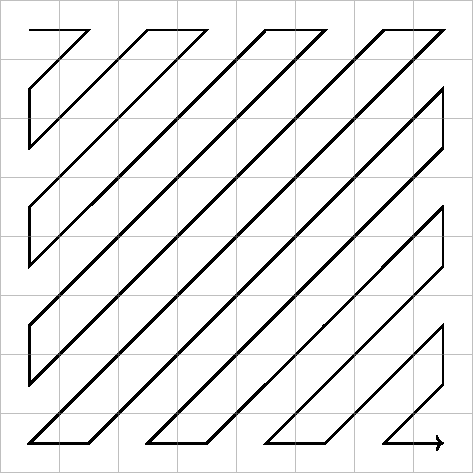
\includegraphics[height = 6cm]{figures/zig-zag.pdf}
    % \caption{} % \label{}
\end{figure}
To reconstruct the image, we can reverse the process:
\begin{enumerate}
    \item Reconstruct the quantised coefficients into an \(8 \times 8\)
          matrix.
    \item Multiply the coefficients by the quantisation matrix.
    \item Compute the inverse DCT of the coefficients.
    \item Repeat for each block.
\end{enumerate}
\section{Deep Learning}
Deep learning allows computational models that are composed of multiple
processing layers to learn representations of data with multiple levels
of abstraction. Deep learning methods discover intricate structure in
large data sets by using the backpropagation algorithm to indicate how
a machine should change its internal parameters that are used to
compute the representation in each layer from the representation in the
previous layer. Deep learning is used in a variety of applications,
including computer vision, speech recognition, natural language
processing, and audio recognition.
\subsection{Supervised Learning}
Supervised learning is the machine learning task of learning a function
that maps an input to an output, based on example input-output pairs.
It infers a function from labelled training data consisting of a set of
training examples. In the training phase, the model is trained to
minimise the error between the predicted output and the true output,
called the \textbf{loss function}. The model can then be evaluated on
unseen test data to determine how well it generalises to new data.
\subsubsection{Nearest Neighbours Classifiers}
A simple image classifier is the nearest neighbours classifier, which
classifies an image by comparing it to labelled training images and
finding the class it is most similar to. This algorithm transforms all
images into an image embedding space, where images are represented by
an \(N \times M\)-d vector of all pixel intensities. To determine if
images are similar, we can use a similarity metric such as the
Euclidean distance or the cosine similarity.
\subsubsection{Linear Classifiers}
A linear classifier makes predictions by dividing the input space into
regions separated by hyperplanes. The model computes a weighted sum of
the input features and compares it to a threshold to make a prediction.
The model can be represented as:
\begin{equation*}
    \symbf{y} = \symbf{W}^\top \symbf{x} + \symbf{b}
\end{equation*}
where \(\symbf{W} \in \R^{K \times p}\) is the weight matrix,
\(\symbf{x} \in \R^p\) is the input feature vector, and
\(\symbf{b} \in \R^K\) is the bias term. Here, \(K\) is the
number of classes and \(p\) is the number of features. The output vector
\(\symbf{y}\) is a vector of unnormalised log-probabilities for each
class. The class with the highest score is the predicted class. To
introduce non-linearity into the model, we often use an activation
function \(a\) on the output of the linear model:
\begin{equation*}
    \symbf{z} = a\left( \symbf{W}^\top \symbf{x} + \symbf{b} \right),
\end{equation*}
where the activation function is typically the Rectified Linear Unit
(ReLU) function:
\begin{equation*}
    a\left( x \right) = \mathrm{ReLU}\left( x \right) = \max\left( 0,\: x \right),
\end{equation*}
or other functions such as the sigmoid or hyperbolic tangent functions:
\begin{align*}
    a\left( x \right) & = \sigma\left( x \right) = \frac{1}{1 + e^{-x}},             \\
    a\left( x \right) & = \tanh\left( x \right) = \frac{e^x - e^{-x}}{e^x + e^{-x}}.
\end{align*}

To learn the coefficients in \(\symbf{W}\) and \(\symbf{b}\) we can use
a \textbf{loss function} to measure the quality of the model's
predictions. A common loss function is the \textbf{cross-entropy loss},
which measures the difference between the predicted class probabilities
and the true class probabilities. The cross-entropy loss for a single
training example is given by:
\begin{equation*}
    L^{\left( i \right)} = -\log{\left( \frac{e^{y_i}}{\sum_j e^{y_j}} \right)} = -y_i + \log{\sum_j e^{y_j}}.
\end{equation*}
Here we are talking the logarithm of the softmax function, which is a
generalisation of the logistic (sigmoid) function that can be used for
multi-class classification. The softmax function is defined as:
\begin{equation*}
    \sigma \left( \symbf{y} \right)_i = \frac{e^{y_i}}{\sum_j e^{y_j}}.
\end{equation*}
The cross-entropy loss for the entire training set is called the cost
which is the average of the loss over all \(n\) training examples:
\begin{equation*}
    J = \frac{1}{n} \sum_{i = 1}^n L^{\left( i \right)}.
\end{equation*}
Given this cost function, we can use a gradient-based optimisation
algorithm to tune the weights and biases of the model to minimise the
cost. One common optimisation algorithm is \textbf{stochastic gradient
    descent} (SGD):
\begin{align*}
    \symbf{W} & \gets \symbf{W} - \eta \pdv{J}{\symbf{W}}, \\
    \symbf{b} & \gets \symbf{b} - \eta \pdv{J}{\symbf{b}},
\end{align*}
where \(\eta\) is the learning rate. To take advantage of computing
capability, we can introduce many layers into the model to create a
fully connected neural network.
\subsubsection{Convolutional Neural Networks (CNNs)}
When classifying images, we can use convolution kernels to learn
features from the image data. Convolutional Neural Networks (CNNs) are
a type of neural network that is well-suited to image classification
tasks. CNNs use convolutional layers to learn features from the input
image, and pooling layers to reduce the spatial dimensions of the
feature maps. A convolution layer has 4 hyperparameters:
\begin{itemize}
    \item Number of filters \(K\)
    \item Filter size \(F\)
    \item Stride \(S\)
    \item Padding \(P\)
\end{itemize}
Given an input of dimension \(N \times M \times C\), the output has a
dimension of \(N' \times M' \times K\), where:
\begin{align*}
    N' & = \frac{N - F + 2P}{S} + 1, \\
    M' & = \frac{M - F + 2P}{S} + 1.
\end{align*}
The number of parameters is \(F^2 CK\) with \(K\) biases. A pooling
layer is often applied after a convolutional layer to reduce the spatial
dimensions of the feature maps.
\subsubsection{Training}
Each update step in the backpropagation algorithm can be performed in
batches or on the entire training set depending on hardware
availability. An \textbf{epoch} is a single pass through the entire
training set. The number of updates in an epoch refers to the number of
batches required to cover the entire training set:
\begin{equation*}
    \text{updates per epoch} = \frac{n}{b},
\end{equation*}
where \(b\) is the batch size. To decide which epoch to stop training,
we can use a validation set to monitor the model's performance. This set
is not used to train the model, but to evaluate the model's performance
on unseen data, on every epoch. A plot of the training and validation
loss for each epoch, can be used to determine when to stop training.
\subsubsection{Gradient Descent Optimisation}
If the number of training examples is large, it may be infeasible to
apply gradient descent on the entire training set. We can instead
consider the following variants of the gradient descent algorithm we
saw earlier:
\begin{itemize}
    \item \textbf{Batch Gradient Descent}: Weights are updated using the
          gradients of the entire training set. This method is slow and
          computationally expensive.
    \item \textbf{Stochastic Gradient Descent (SGD)}: Weights are updated
          using the gradients of a single training example. This method
          is noisy and may not converge to the global minimum.
    \item \textbf{Mini-Batch Gradient Descent}: Weights are updated using
          the gradients of a small subset of the training set. This
          method is faster than batch gradient descent and less noisy
          than stochastic gradient descent.
\end{itemize}
To further improve these algorithms, we can introduce momentum to
accelerate convergence and reduce oscillations around local minima.
The momentum algorithm is defined as:
\begin{align*}
    \symbf{v} & \gets \rho \symbf{v} + \pdv{J}{\symbf{w}}, \\
    \symbf{w} & \gets \symbf{w} - \eta \symbf{v},
\end{align*}
here \(\symbf{w}\) represents both the weights and biases in the model.
The addition of a velocity term \(\symbf{v}\) allows the model to build
up velocity as a running mean of the gradients. The hyperparameter
\(\rho\) controls the momentum term by adding friction, and is typically
set to a value between 0.9 and 0.99. Other more advanced optimisation
algorithms include the Nesterov Accelerated Gradient (NAG), AdaGrad,
RMSprop, and Adam optimisers. These algorithms use adaptive learning
rates to improve convergence and generalisation. We can also use
learning rate schedules to adjust the learning rate during training.
\end{document}

